\documentclass[12pt, a4paper, oneside]{book}

%---------------------------------------------------------   
\usepackage[english,romanian,magyar]{babel}       
\usepackage[utf8]{inputenc}
\usepackage[a4,center,axes]{crop}
\usepackage{calc}
\usepackage{t1enc}
\usepackage{amsthm}
\usepackage{rotating}
\usepackage{amssymb}
\usepackage{lscape}
\usepackage{anysize}
\usepackage{setspace} 
\usepackage{comment}
\usepackage{graphicx}
\usepackage{setspace} 
\usepackage{tocloft}
\usepackage{indentfirst}
\usepackage{url}
\usepackage[top=3cm, bottom=2cm, left=3cm, right=2cm]{geometry}

%---------------------------------------------------------
%%
%%
%% alapformázások
%%
%%
\sloppy                        % sorkizárás kezelése
\clubpenalty = 10000           % árvasorok
\widowpenalty = 10000          % fatyúsorok
\raggedbottom                  % függõleges kizárás az oldalon
\setcounter{secnumdepth}{3}    % alcimek számozási mélysége
\setcounter{tocdepth}{3}       % tartalomjegyzék mélysége
\brokenpenalty = 10000         % lap aljai elválasztások tiltása
\doublehyphendemerits = 80000  % egymást követõ elválasztások

%\marginsize{2cm}{2cm}{2cm}{2cm} %marók beállítása
\onehalfspacing %sorközök megaddása

\theoremstyle{tetel}
\newtheorem{mydef}{értelmezés}[chapter]
\newtheorem{megj}{megjegyzés}[chapter]

\def\partro#1{\foreignlanguage{romanian}{\addcontentsline{tro}{part}{%\if@mainmatter\protect\numberline{\thechapter.}\fi
\MakeUppercase{#1}}}}
\def\chapterro#1{\foreignlanguage{romanian}{\addcontentsline{tro}{chapter}{\if@mainmatter\protect\numberline{\thechapter.}\fi#1}}}
\def\sectionro#1{\foreignlanguage{romanian}{\addcontentsline{tro}{section}{\protect\numberline{\thesection.}#1}}}
\def\subsectionro#1{\foreignlanguage{romanian}{\addcontentsline{tro}{subsection}{\protect\numberline{\thesubsection.}#1}}}
\def\subsubsectionro#1{\foreignlanguage{romanian}{\addcontentsline{tro}{subsubsection}{\protect\numberline{\thesubsubsection.}#1}}}

%roman tartalom def
%---------------------------------------------------------
\newcommand{\nombreindice}{Cuprins}
\newlistof{indice}{tce}{\nombreindice}

\newcommand\capterro[1]{%
  \addcontentsline{tce}{chapter}{\protect\makebox[1.3em][l]{\thechapter.}#1}}
\newcommand\secro[1]{%
  \addcontentsline{tce}{section}{\protect\makebox[2.8em][l]{\thesection.}#1}}
\newcommand\ssecro[1]{%
\addcontentsline{tce}{subsection}{\protect\makebox[3em][l]{\thesubsection.}#1}}

%angol tartalom def
%---------------------------------------------------------

\newcommand{\tcontents}{Table Of Contents}
\newlistof{indiceen}{tcen}{\tcontents}

\newcommand\capteren[1]{%
  \addcontentsline{tcen}{chapter}{\protect\makebox[1.3em][l]{\thechapter.}#1}}
\newcommand\secen[1]{%
  \addcontentsline{tcen}{section}{\protect\makebox[2.8em][l]{\thesection.}#1}}
\newcommand\ssecen[1]{%
\addcontentsline{tcen}{subsection}{\protect\makebox[3em][l]{\thesubsection.}#1}}

%---------------------------------------------------------
\newcommand*{\field}[1]{\mathbb{#1}}

%---------------------------------------------------------

%---------------------------------------------------------
\begin{document}
\pagenumbering{arabic}

%magyar borito
%--------------------------------------------------------
\newpage
\thispagestyle{empty}
\begin{center}
    \Large SAPIENTIA ERDÉLYI MAGYAR TUDOMÁNYEGYETEM\\
    \Large MŰSZAKI ÉS HUMÁNTUDOMÁNYOK KAR, MAROSVÁSÁRHELY\\
    \Large SZOFTVERFEJLESZTÉS SZAK\\
\end{center}

\begin{center}
 	\vspace{2cm}\LARGE \textbf{Hibrid képleírás 2.0}\\
	 \vspace{1cm}\LARGE \textbf{MESTERI DISSZERTÁCIÓ}\\
\end{center}

\vspace{2cm}
\begin{figure}[htb]
\hspace{5.7cm}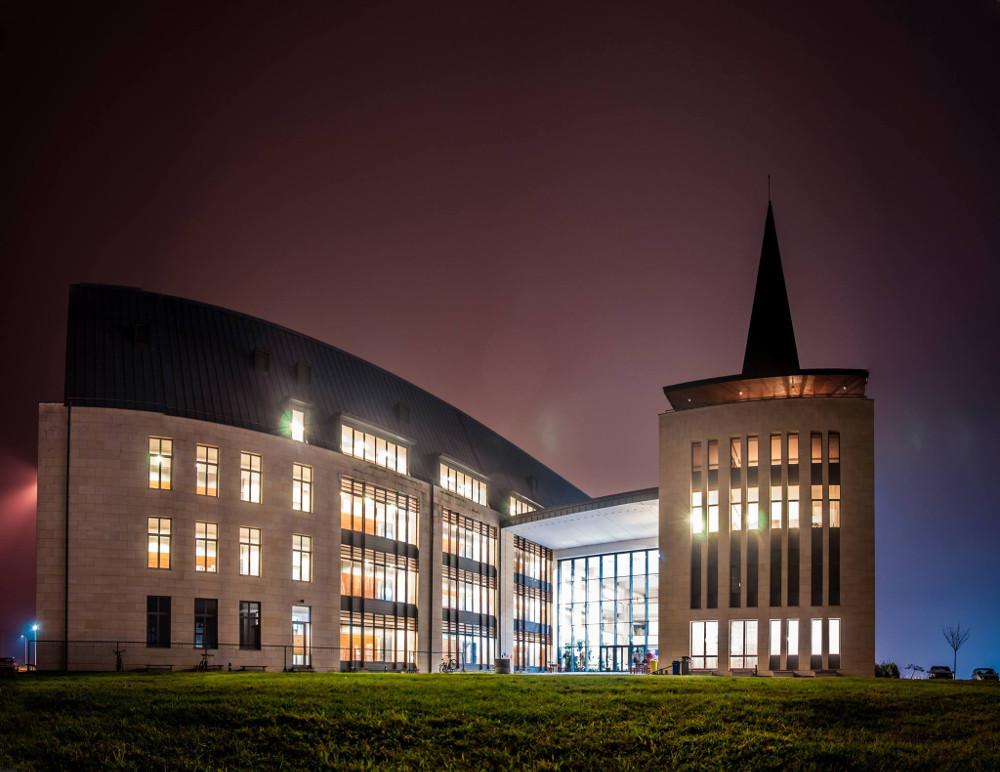
\includegraphics[bb = 0 0 160 160]{sapi.jpg}
\end{figure}

\vspace{2cm}
\begin{center}
\begin{tabular}{lcccccccccccl}
    TÉMAVEZETŐ:&&&&&&& &&&&&SZERZŐ:\\
     dr. Egyed-Zsigmond Előd&&&&&& &&&&&&Madaras Hunór\\
	Egyetemi Docens
\end{tabular}
\end{center}

\begin{center}
    \vspace{0.5cm}\textbf{2016 Június}
\end{center}
\vspace*{\fill}
%roman borito
%-------------------------------------------------------------
\newpage
\thispagestyle{empty}
\begin{center}
    %\Large UNIVERSITATEA BABE\c{S}-BOLYAI CLUJ-NAPOCA\\
    \Large UNIVERSITATEA SAPIENTIA TÂRGU-MURE\c{S}\\
    \Large FACULTATEA DE \c{S}TIIN\c{T}E TEHNICE \c{S}I UMANISTE\\
    \Large SPECIALIZAREA DEZVOLTARE DE SOFTWARE\\
\end{center}

\begin{center}
    \vspace{3cm}\LARGE \textbf{Descrierea hibridã a imaginilor 2.0}\\
    \vspace{1cm}\LARGE\textbf{Lucrare de master}\\
\end{center}

\vspace{2cm}
\begin{figure}[htb]
\hspace{5.7cm}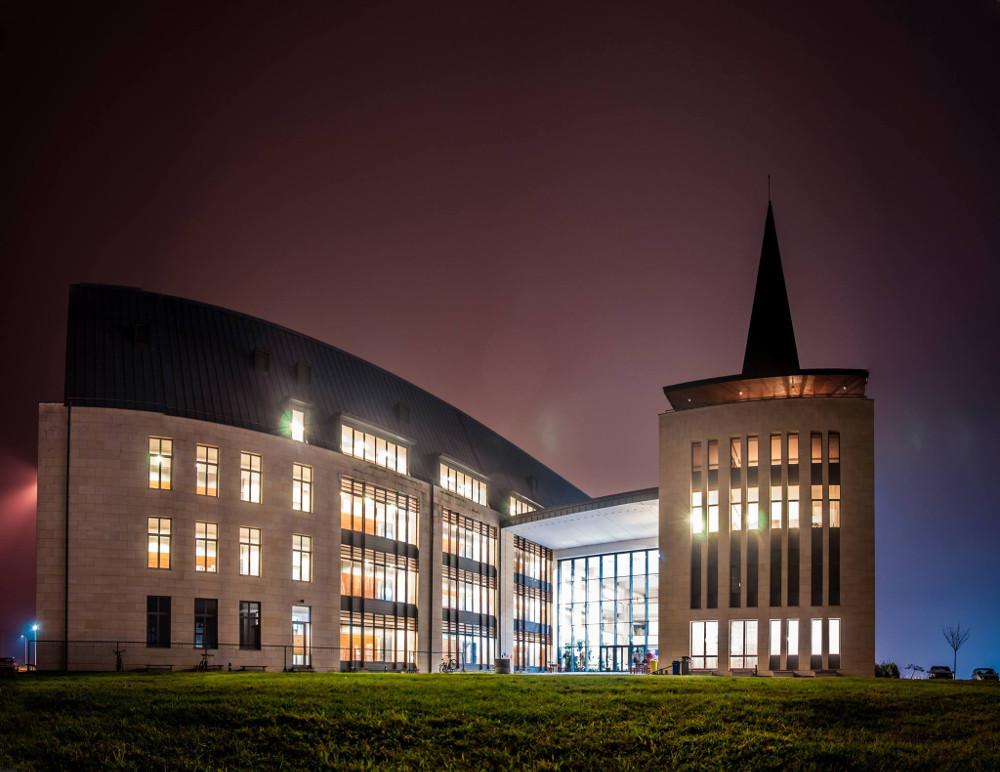
\includegraphics[bb = 0 0 160 160]{sapi.jpg}
\end{figure}

\vspace{2cm}
\begin{center}
\begin{tabular}{lcccccccccccl}
    Coordonator \c{s}tiin\c{t}ific:&&&&&&& &&&&&Absolvent:\\
     dr. Egyed-Zsigmond Előd&&&&&& &&&&&&Madaras Hunór\\

\end{tabular}
\end{center}

\begin{center}
    \vspace{1cm}\textbf{2016 Iunie}
\end{center}

%angol borito
%-------------------------------------------------------------

\newpage
\thispagestyle{empty}
\begin{center}
    %\Large BABE\c{S}-BOLYAI UNIVERSITY CLUJ-NAPOCA\\
    \Large SAPIENTIA UNIVERSITY TÂRGU MURE\c{S}\\
    \Large FACULTY OF TECHNICAL AND HUMAN SCIENCES\\
    \Large SOFTWARE DEVELOPMENT SPECIALIZATION\\
\end{center}

\begin{center}
    \vspace{3cm}\LARGE \textbf{Hybrid image description 2.0}\\
    \vspace{1cm}\LARGE \textbf{Master Thesis}\\
\end{center}

\vspace{2cm}
\begin{figure}[htb]
\hspace{5.7cm}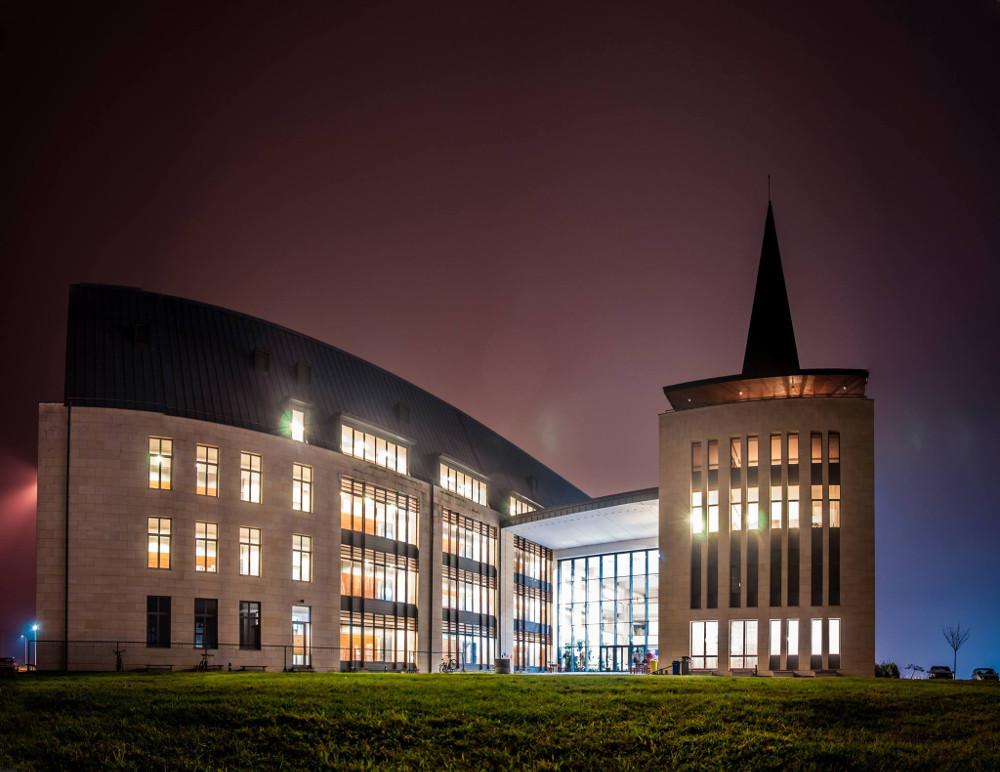
\includegraphics[bb = 0 0 160 160]{sapi.jpg}
\end{figure}

\vspace{2cm}
\begin{center}
\begin{tabular}{lcccccccccccl}
     Advisor: & & &&&& &&&&&& Student:\\
     dr. Egyed-Zsigmond Előd &&&&&& &&&&&& Madaras Hunór\\
\end{tabular}
\end{center}

\begin{center}
    \vspace{1cm}\textbf{2016 June}
\end{center}

%eredetisegi nyilatkozat
%-------------------------------------------------------------
\newpage
\thispagestyle{empty}
eredetisegi nyilatkozat
%kivonat magyar
%-------------------------------------------------------------
\newpage
\thispagestyle{empty}
\begin{center}
    \Large KIVONAT
\end{center}

	 A mindennapi életben rengeteg információval találkozunk, a legjobban a képek alapján maradnak meg ezek az adatok nekünk. Az emberek egyszerűen fel tudják ismerni a képeken látható információt, tárgyakat, embereket, tájakat, viszont a számítógépeknek ehhez tanulás kell. Manapság egy kép élettartama 24 óra, sok képet készítünk és hamar el is feledkezünk róluk. Mi történne, ha lenne egy olyan rendszerünk, ami képes nekünk szavak alapján előkeresni a képeket, felismerni az információt rajtuk és úgy rendezni őket.

	A kutatás célja egy olyan rendszert felállítani, tökéletesíteni, mely képes egy általunk választott képre megmondani, hogy egy kulcsszó milyen valószínűséggel szerepel a képen (Például a kulcsszó legyen a szék és a rendszer megmondja, hogy a képünkön van e szék vagy nincs). Lényegében a cél a kulcsszavak és képek közötti összefüggések megtanulása. Ehhez a képleírást két szempontból közelítem meg. 
Az első, a képekhez rendelt kulcsszavak, a második, a már jól ismert pixel alapú képleírás. A képeket és a kulcsszavakat különböző publikus adatbázisokból lehet elérni, például a Flickr\cite{1}, Getty Images\cite{2}, ImageNet\cite{3}, ezáltal már kapunk olyan képeket, melyek le vannak írva szavakkal, az az tulajdonságok vannak rendelve a képekhez. A második megközelítés a pixel alapú képleírás. Tudjuk, hogy a képtartalom karakterizálható numerikus leírás vektorok segítségével. Ezek a vektorok különféle algoritmusok eredményei, ilyen például a különböző hisztogramok, érdekes pontok, textúra leírás vagy a kontúr. 

	A projekt célja a leírásvektorok és a kulcsszavak közötti összefüggések felismerése, megtanulása, például melyek, azok a képleírás típusok, amelyek legjobban eldöntik, hogy az illető kép kint vagy bent volt készítve, van-e arc a képen, vannak-e állatok rajta? Fő cél, hogy egy új, még kulcsszavakkal le nem írt, képhez megtaláljuk a legtalálóbb kulcsszavakat egy adott kulcsszó halmazból. Ennek a megvalósításához be kell tanítsuk a rendszert, modelleket kell felállítani, határértékeket kell rendeljünk a kulcsszavakhoz, annak függvényében, hogy egy képleíró módszer, tanulás modell, mennyire diszkrimináns az illető kulcsszóra nézve. Rendelkezünk egy 50.000 képet és azok háromnyelvű leírását tartalmazó adatbázissal. Ezt az adatbázist a Flickr\cite{1} és Getty Images\cite{2} képbank weboldalairól töltöttük le. Valamint még van egy 82.000 kulcsszó halmazt tartalmazó adatcsomagunk a hozzájuk tartozó kép címekkel az ImageNet-ről\cite{3}. Célunk eléréséhez szűréseket kell végezni a képeken, például kulcsszavak alapján, tanítani a rendszer osztályozó algoritmusok segítségével, tanuló modelleket kell felállítani, hogy ezek alapján határértékeket tudjunk meghatározni a kulcsszavakra.

Összefoglalóban, a kutatás célja, hogy egy képről eldöntsük, hogy egy adott halmazból származó kulcsszó milyen valószínűséggel írja le és ehhez szükségünk van nem kizárólag egy képleíró algoritmusra és osztályozó módszerre, hanem akár ezek kombinációjára.


\begin{flushright}
\textbf{Madaras Hunór,}\\
.........................
\end{flushright}

%kivonat roman
%-------------------------------------------------------------
\newpage
\thispagestyle{empty}
\begin{center}
    \Large ABSTRACT
\end{center}

	În vița de zi cu zi ne întâlnim cu foarte multe informații, acestea sunt memorate cel mai bine pe baza imaginilor. Informațiile de pe imagini adică peisajele, obiectele sunt recunoscute ușor de către oameni, dar calculatoarele au nevoie de un proces de învățare. În zilele noastre viața unei imagini nu depășește 24 de ore, facem multe fotografii și uităm repede de ele. Ce s-ar întâmpla dacă am avea un sistem informatic care ar recunoaște informațiile de pe imagini și le-ar procesa după criteriile date de către utilizatori?

	Scopul cercetării noastre este construirea unui sistem informatic, care poate determina probabilitatea prezenței unui element cheie din imagine. În principiu, scopul este învățarea legăturilor dintre cuvinte cheie și imagini. Pentru acest scop abordez descrierea hibridă din două puncte de vedere.

	Primul punct de vedere este atribuirea cuvintelor cheie la imagini și al doilea este descrierea imaginilor pe bază de pixeli.  Pozele și cuvintele cheie provin din baze de date publice, de exemplu Flickr\cite{1}, Getty Images\cite{2}, ImageNet\cite{3}. Astfel putem deține imagini care sunt deja descrise cu cuvinte cheie. A doua abordare este descrierea imaginilor pe bază de pixeli. După cum știm conținutul pozelor se poate caracteriza prin descriere numerică dată de vectori. Vectorii menționați mai înainte, sunt rezultatul diferitelor algoritmi, de exemplu histograme, descrierea conturilor și a texturilor.

	Obiectivul proiectului este identificarea și învățarea legăturii dintre vectori de descriere și cuvintele cheie, de exemplu care sunt tipurile de descriere hibridă care determină dacă poza a fost fotografiată înauntru sau afară, dacă apar animale sau fețe în poze. Scopul este ca pentru o imagine nouă, încă nedescrisă de cuvinte cheie, să găsim cuvintele cheie cele mai potrivite dintr-o mulțime de cuvinte cheie date. Pentru realizare sunt necesare următoarele: învățarea sistemului informatic, stabilirea unui model, atribuirea limitelor la cuvinte cheie, în funcție de tipul modelului și cât de discriminant este pentru cuvântul cheie ales. Avem la dispoziție 50.000 de poze și o bază de date care conține descrierea acestora în trei limbi. Baza de date a fost descărcată de pe site-urile web ale băncilor de imagini Flickr\cite{1} și Getty Images\cite{2}. Pe lângă acesta avem un pachet de date care conține 82.000 de cuvinte cheie alăturate titlului imaginilor de pe ImageNet\cite{3}. Pentru obținerea scopului este necesar filtratea imaginilor, de exemplu pe baza cuvintelor cheie, învățarea cu ajutorul sistemului de clasificare a algoritmilor și stabilirea modelelor de învățare prin care putem calcula limita pentru cuvintele cheie.

	Prin urmare, scopul lucrării noastre este să stabilim probabilitatea cu care un cuvânt cheie, aparținând unei mulțimi date, descrie o imagine. Pentru acesta este necesar nu numai un algoritm de descriere a imaginilor ci și un model de clasificare dar și combinarea acestora.

\begin{flushright}
\textbf{Madaras Hunór,}\\
.........................
\end{flushright}

%kivonat angol
%-------------------------------------------------------------
\newpage
\thispagestyle{empty}
\begin{center}
    \Large ABSTRACT
\end{center}

	In everyday life we meet a lot of information, the most of them remains based on what we see on the images. People simply can recognize the information displayed on pictures, like objects, people, landscapes, but computers have to learn for this feature. Nowadays a picture's lifetime is 24 hours, we take a lot of pictures and forget them fast. What would happen if we would have a system that is able to look for pictures, based on words, for us and recognize the objects on them. For example, let the keyword be the chair and the system will tell you that on the picture is chair or not.

	Our research aims to establish and to improve a system that is able to say about a chosen picture the probability that a keyword describes it or not. For example, let the keyword be the chair and the system will tell you that on the picture is chair or not. In essence, the goal is to find and learn the relationship between keywords and pictures. For this we approach the image description from two different points of views. On one hand, based on image metadata: keywords attached to the images, on the other hand the image content. Images and keywords are available from several public repositories and websites like Flickr\cite{1}, Getty Images\cite{2}, ImageNet\cite{3}. These provide a large number of tagged images. In order to get information from the images, the content, we calculate description vectors based on image features, by several well-known algorithms. These algorithms are the different kinds of histograms, interest points like the SIFT descriptor, different texture and contour descriptors.

	The goal of our project is to learn the relations between keywords and image features based on a large number of annotated images in order to be able to provide a relation measure between a new image and a keyword. In order to achieve this objective, we have to train the system, set up models, calculate thresholds and assign them to the words, depending on how discriminant is a learning method, a training model. We have a database with 50.000 images, with their description (words) in three languages. This database was downloaded from Flickr \cite{1} and Getty Images \cite{2}. Also, there is a data packet containing 82.000 keyword aggregation, associated with image URLs from the ImageNet\cite{3}.

	The summary of the research is to determine a probability for keywords, from a given list, with what probability each decribes a given image, and for this we need not only an image describing algorithm and classification method, but even a combination of these.


\begin{flushright}
\textbf{Madaras Hunór,}\\
.........................
\end{flushright}

%tartalom jegyzek
%-------------------------------------------------------------
\newpage
\tableofcontents
\newpage
\listofindice
\newpage
\listofindiceen

\selectlanguage{magyar}

%-------------------------------------------------------------
\chapter{Bevezető}
\capterro{Întroducere}
\capteren{Indroduction}

	Napjainkban a képfeldolgozás nagyon elterjedt tudomány és kutatási terület is egyben. A képfeldolgozás általában pixel alapján történik, ezek segítségével nyerünk ki információkat a képekből. Egyik legegyszerűbb pixel alapú információ kinyerés az a hisztogram számítás, vagyis meghatározni, hogy minden színárnyalat hányszor fordul elő a képen. Különböző hisztogramok léteznek, mint például szín(RGB, R, G, B), luminance(fényesség), szürke hisztogram. Vannak ennél összetettebb hisztogram számítási módszerek, mint például CEDD(Color and Edge Directivity Descriptor), FCTH(Fuzzy Color and Texture Histogram) és még egy pár, melyek jól elkülöníthető információt adnak egy képről. 

	Más pixel alapú feldolgozási szempont lehet az érdekes pontok, textúra elemzés, él detektálás. Vannak képmegosztó oldalak (kép bankok, Flickr \cite{1}, Getty Images \cite{2}) ahol a felhasználóknak lehetőségük van a feltöltött képekhez kulcsszavakat adni, ez által a képek olyan leírásokkal fognak rendelkezni, mely minden embernek érthető lesz, hisz szavakkal íródnak le. Az előbb említett kép bankok közé tartozik az ImageNet \cite{3} is, ahol a képek WordNet \cite{15} hierarchiája, osztályozása, (jelenleg csak a főnevek) alapján vannak rendezve, viszont nagyon jó és pontos kép-kulcsszó adatbázissal rendelkezik. Ezeket figyelembe véve lehetőségünk van két szempontból jellemezni, feldolgozni a képeket. A pixel alapú képfeldolgozással, amikor a képpontokkal dolgozunk és a kulcsszavak alapján, amikor a hozzájuk rendelt leírás alapján hasonlítjuk össze, szűrjük őket. 

	A jelenlegi kutatás már egy továbbfejlesztett változat. A problémával foglalkoztam már alapképzésen és az akkori eredményekből kiindulva, azokra építve, fejlesztettem a rendszert. Próbáltuk kiküszöbölni azokat a problémás helyeket és néhány helyen új megközelítést alkalmaztunk. Ilyen például a tanulási fázis. 

	A kutatás első részében a képek pozitív és negatív hisztogramjait egy szűrés alá vetettük, amelyből megkaptuk a legjellemzőbbeket és a legkevésbé jellemzőeket, majd ezekből különböző átlagolási algoritmusok segítségével pozitív és negatív leírásvektorokat állítottunk elő és ezekeket használtuk fel egy új kép leírásánál. A kutatás jelenlegi fázisában a tanulásba bevezettünk, osztályozó algoritmusokat, modelleket és kombináltuk őket a képleíró módszerekkel, majd a tanulás pontossága alapján határoztuk meg a módszer modelleket, amelyek a legjobbak egy kulcsszóra nézve. Erre szükség volt mivel úgy tapasztaltuk, hogy a kutatás első részében kiszámolt átlag leírásvektorok nem elég pontosak. 

	Valamint a képek pontosságán is javítottunk, mivel az előző adatbázisban (Flickr \cite{1}, Getty Images \cite{2}) a kulcsszavakhoz tartozó képek túl átlagosnak bizonyultak, ezért vezettük be és kombináltuk a kulcsszavakat és képeket az ImageNet \cite{3} adatbázisával, mely sokkal pontosabb és strukturáltabb.

	Az elkövetkezendőkben bemutatásra kerülnek az előző kutatás szempontjai, a képfeldolgozási algoritmusok, a kulcsszavak és a képek közti kapcsolatot, a szabályok melyeket felállítottunk, a következtetések melyeket levontunk és az újító módszerek a régiekhez képest.


%-------------------------------------------------------------
\chapter{A rendszer}
\capterro{Sistemul}
\capteren{The system}

%-------------------------------------------------------------
\section{Áttekintés}
\secro{Privire de ansamblu asupra}
\secen{Overview}

	Az egész az adatok rendezésével kezdődik. Amint azt a \ref{felulnezet_1} ábrán is láthatjuk az első lépés az, hogy átadjuk a rendszernek a képleíró módszereket (a LIRE (Lucene Image Retrieval)\cite{8} könyvtárcsomagot használtuk, a következő fejezetekben lesz róla szó bővebben) és az adatbázist a kulcsszavakkal és a hozzájuk tartozó képekkel.  Ez maga az előkészítés a tanulásra. A jelen folyamat azt mutatja be, hogy hogy történik egy kulcsszó megtanulása. 

	A második lépés abból áll, hogy a rendelkezésünkre álló képeket felosztjuk a tanulni kívánt kulcsszó alapján két halmazra. Az egyik halmazba kerülnek, azok a képek melyeket leír a kulcsszó és a másikba azok a képek melyeket nem ír le a kulcsszó. Vagyis egy-egy halmaz a pozitív és egy a negatív képekkel. 
A harmadik lépésben, a két halmazban szereplő képekre kiszámoljuk a leírásvektorokat, az összes rendelkezésünkre álló képleíró módszer alapján. Ez az egyik időigényesebb feladat a tanulás folyamatában, ezért a már kiszámolt leírásvektorokat elmentjük és felhasználjuk a következő kulcsszavak tanulásánál is, így időt takarítunk meg.

	A negyedik fázis már a tanulásról szól és ez a legbonyolultabb, leg időigényesebb része az egész mechanizmusnak. A tanuláshoz, osztályozáshoz a Weka \cite{16} könyvtárcsomagot használtuk, hogy milyen osztályozó algoritmusokat, módszereket alkalmaztunk arról a következő fejezetekben lesz szó. Erről a fázisról azt kell tudni, hogy a képleíró módszereket és az osztályozó modelleket kombináltuk, minden módszer minden modellel, lényegében párokat képeztünk a módszerekből és a modellekből és ezek alapján történt a tanulás. 

	Az ötödik lépésben a megtanult módszer modelleket osztályoztuk, rendeztük csökkenő sorrendbe, a tanulás pontossága alapján. A teszt képeket a tanuló képekből vettük ki és egy tízszeres cross validation-t \cite{17} alkalmaztunk az egyedi esetek kiszűrése érdekében. Ezt a pontosságot felhasználva megkaptuk, hogy egy módszer modell mennyire tanult jól, mennyire volt hatékony. 

	A hatodik szakasz a legjobb módszer modellek kiválasztásáról szol. Itt egy várt bemeneti paraméter alapján a rendezett listából kiválasztjuk a legeslegnagyobb pontossággal rendelkező $OL$ darab módszer modellt. Ezek a kiválasztott elemek lesznek a legdiszkriminánsabb módszer modellek a tanult kulcsszóra nézve. A kiválasztott komponenseket elmentjük egy adatbázisba, melyeket majd felhasználunk egy új kép elemzésénél, hogy megtudjuk, hogy a megtanult kulcsszó leírja-e az új képet vagy sem. 

\begin{figure}[h]
\begin{center}
\includegraphics[scale=0.6]{felulnezet_1.jpg}
\caption{{A tanulás lépései felülnézetből}}
\label{felulnezet_1}
\end{center}
\end{figure}

	A \ref{felulnezet_2} ábrán a valószínűség számítás látható, a fázis amikor egy új képről el kell dönteni, hogy egy megtanult kulcsozó leírja e a képet és hogy milyen valószínűséggel. 

	Az első lépésben a kiválasztott kulcsszó alapján kivesszük az adatbázisból a hozzá tartozó megtanult legdiszkriminánsabb módszer modelleket. Ezek után a kapott modellekhez tartozó, képleíró módszerek alapján leírásvektorokat számítunk az új képre. 

	A második lépésben van egy adatstruktúránk, ami tartalmazza a megtanult eredményeket és az új kép leírásvektorait módszer modellenként.

	A harmadik fázis a kiértékelésről szól. Itt számoljuk ki a végső valószínűséget, amely alapján eldönthetjük, hogy az érdekelt kulcsszó leírja-e a képet vagy sem. Amint látható, módszer modellenként számítunk valószínűséget, a Weka \cite{16} egyik  erre írt függvénye segítségével, melyről a következő fejezetekben lesz szó. Miután minden elemre megvan a külön-külön a valószínűség, ezeket összeadjuk és elosztjuk a módszer modellek számával, vagyis $OL$-el, így kapjuk meg a végső valószínűséget.
	
\begin{figure}[h]
\begin{center}
\includegraphics[scale=0.6]{felulnezet_2.jpg}
\caption{{A valószínűség számítás felülnézetből}}
\label{felulnezet_2}
\end{center}
\end{figure}

%-------------------------------------------------------------
\newpage

\section{A diszkrimináns módszer modellek meghatározása}
\secro{Determinarea modelelor si metodelor discriminante}
\secen{Determination of the discriminant method models}

%-------------------------------------------------------------
\subsection{Előkészítő módszer}
\ssecro{Metoda preparării}
\ssecen{Preparation method}

	Legyen $TK$ a tanuló képek halmaza, úgy hogy $TK$ = \{ $kep_i$, $Ksz_i$ \}, ahol $kep_i$ egy kép és $Ksz_i$ a $kep_i$-hez tartozó kulcsszavak halmaza, $MK$ a képleíró módszerek halmaza, $\mid TK \mid$ = $N$ és $\mid MK \mid$ = $M$. A mostani kutatási fázisban nem szükséges a képek között távolságot számolni, szűrést végezni, mivel a tanuló képek pontosak. A jelenlegi kép–kulcsszó  adatbázis az ImageNet-ről \cite{3} van, ahol sokkal pontosabb érték párok vannak, mint a Flickr \cite{1} és Getty Images \cite{2} adatbázisaiban. Az előző verzióban a már meglévő $N$ darab képből felépítettünk minden módszerre egy $T_j$ = $N$ x $N$ mátrixot, ahol $T_j(a,b)$ = $m_j$(a,b) (két kép közötti távolság az $m_j$ képleíró módszerrel és $a,b \in {TK} $), $j \in 1\dots M$. A $T_j(a,b)$ távolság, képleírás vektor alapú és általában a koszinusz távolságra épül.

	Erre azért volt szükség, mert ezek alapján választottuk ki azokat a hisztogramokat melyek segítségével kaptuk meg a legjellemzőbb és a legkevésbé jellemző leírásvektorokat. Így biztosak lehettünk abban, hogy a legjobb képeket választjuk ki (a legjobb leíró és a legkevésbé leíró) a végső vektorok meghatározására.

%-------------------------------------------------------------
\subsection{Tanulás}
\ssecro{Învăţare}
\ssecen{Learning}

Mivel szükségünk van, minden kulcsszóra külön-külön és nem kulcsszó halmazokra, ahogy az megtalálható a $TK$ halmazban, ezért kinyerjük a kulcsszavakat a $TK$ halmazból és felépítünk egy $KSZ$ = \{ $ksz$\} halmazt, $\mid KSZ \mid$ = $S$ (ennyi kulcsszó van összesen). A $ksz$ = \{ $L_{ksz}$, $NL_{ksz}$ \}, ahol: 

\begin{itemize}
  \item $L_{ksz}$ = \{  $kep_q$ melyeket a $ksz$ kulcsszó leír \} , q =  1 $\dots \mid L_{ksz} \mid$
  \item $NL_{ksz}$ =  \{  $kep_w$ melyeket a $ksz$ kulcsszó nem ír le\}  , w =  1 $\dots \mid NL_{ksz} \mid$, $NL_{ksz} = N - L_{ksz}$
\end{itemize}

Az első tanulás alkalmával egy kulcsszóra 100 képet használtunk fel. Ami azt jelenti, hogy  $L_{ksz}$ tartalmazott 50, a kulcsszót leíró képet és az  $NL_{ksz}$ 50, a kulcsszót nem leíró képet. Nem akartunk, a képek számán növelni, mivel nagyon specifikusak és kíváncsiak voltunk, hogy kevesebb adattal mennyire lesz gyors és eredményes a tanulás. 

\begin{figure}[h]
\begin{center}
\includegraphics[scale=0.4]{cars_flicker_getty.jpg}
\caption{{Négy kép látható a Flickr \cite{1} és Getty Images \cite{2}) adatbázisokból, melyek az “autó” kulcsszóra jellemzőek}}
\label{cars_flicker_getty}
\end{center}
\end{figure}

\begin{figure}[h]
\begin{center}
\includegraphics[scale=0.4]{cars_imgnet.jpg}
\caption{{Négy kép látható a  az ImageNet \cite{3} adatbázisból, melyek az “autó” kulcsszóra jellemzőek}}
\label{cars_imgnet}
\end{center}
\end{figure}

	Az kutatás előző verziójában 11.600 angol nyelvű kulcsszóval dolgoztunk (amelyek között rengeteg szókapcsolat, általános kifejezés, ige volt, ezek nem voltak relevánsak a konkrét információkra nézve, amelyeket mi keresünk). Minden kulcsszóhoz tartozott körülbelül 2000 leíró kép, melyekkel az volt a baj, hogy túl általánosak voltak. Jelen adatbázisunkban, melyet folyamatosan bővítünk az ImageNet-ről \cite{3}, egyelőre található  80 kulcsszó és hozzájuk 8000 kép, ezeknek a leírás vektoraik már ki vannak számolva.  A képleíró módszerek, leírásvektorok a 2.3 fejezetben láthatóak.

	A kevesebb és specifikus tanuló halmaznak (képeknek) az az előnye, hogy nem kell optimalizálást végezni, a képek között (vagyis kiválasztani a legeslegjellemzőbb és legkevésbé jellemző képeket), mivel sokáig tartana a tanulás 4000 képpel (2000 leíró és 2000 nem leíró). A kutatás első fázisaiban egy szó alapú szűrést, valamint kép távolságszámítást alkalmaztunk, melynek végén a tanuló halmazt 20 képre redukáltuk, ami azt jelenti, hogy volt 10 kép ami leírta a kulcsszavat és 10 mely nem írta le a kulcsszavat. Egy kulcsszó alapú szűrés arra nézve, hogy a képeket mennyi közös kulcsszó köti össze és mennyire távol vagy épp közel állnak a képek egymáshoz egy adott kulcsszó halmazon belül, időt vesz igénybe, ami nem is biztos, hogy releváns mivel a kulcsszavak nem mindig pontosak.  A képek közötti távolság számítás szintén időigényes feladatnak minősül, mivel mindegy egyes képre ki kell számolni a leírás vektort, még azokra is melyeket nem fogunk felhasználni a végső vektor, modell felállításánál, valamint ezen vektorok között távolságokat számítani szinten időt vesz igénybe. 

	Az előrelépés érdekében, próbáltuk ki kevesebb, pontosabb képet. Végeredményben a tanuló halmaz képeinek száma több, csak nem biztos, hogy az $NL_{ksz}$ halmazba tartozó elemek annyira távol álnak a $ksz$-től, mivel véletlenszerűen voltak kiválasztva.

	Amint megfigyelhető a \ref{cars_flicker_getty} ábrán, az autó kulcsszót leíró képek a régi adatbázist használva nem pontosak, megjelenik maga a fogalom, de nem specifikus és meghatározó, valamint olyan kép is előfordul, amelyeken maga a tárgy nincs is jelen, inkább csak utalás van rá. Tény, hogy az első három képkockán megjelenik valamilyen formában az autó, de talán csak az első (bal felső) az, ami használható lenne. A jobb felsőn több autó tető is található de ebből nehéz jó információt kinyerni. A bal alsó jó lenne, de mivel valamilyen hatás (efect) van rajta szintén nehéz használható információt kapni belőle. Az utolsó képen (jobb alsón) ugyan megjelennek az autók, de annyira kicsik, hogy az majdnem fel sem tűnik az embernek.  

	A \ref{cars_imgnet} ábrán már a jelenlegi, ImageNet \cite{3}, adatbázisból látható négy, az autó kulcsszóra jellemző, kép. Megállapítható, hogy sokkal pontosabbak, specifikusabbak, mint az \ref{cars_flicker_getty} ábrán lévők. Van ebben a halmazban is elvont kép, de maga a tárgy megjelenik mindegyiken és jó minőségben. Nincsenek elmosódott képek, nincsenek hatások (efec-ek) rajtuk, valamint ami a legfontosabb, a képek információs központjában az autó szerepel. Ez jó, mert a tanuláshoz megbízható adatokra van szükségünk.

A cél az volt a tanulásnál, hogy felépítsünk minden $ksz$-re olyan módszer modelleket, melyek segítségével majd valószínűséget tudunk számolni egy új képre. A tanuláshoz, osztályozáshoz a Weka \cite{16} könyvtárcsomagot használtuk, mivel ebben megtalálhatóak már különböző osztályozási algoritmusok, mint például J48, DecisionStump. Az osztályozók a 2.4 fejezetben láthatóak. Ezekből az osztályozokból modelleket lehet generálni melyek nagy segítséget nyújtanak az új kép vizsgálatánál.
 
	Jelen helyzetben 16 képleíró módszerrel dolgozunk, ami azt jelenti, hogy 16 féle leírásvektort tudunk kiszámítani egy képre, $M$ = 16. A képleíró módszerek a 2.3 fejezetben láthatóak. 
	
	Az osztályozó algoritmusoknál két megközelítést használtunk. Először négy féle osztályozó algoritmust használunk J48, PART, DecisionTable, DecisionStump, majd bevezettünk még huszonhatot. Azért közelítettünk meg először csak kevesebb osztályozó algoritmussal a problémát, mert kíváncsiak voltunk, hogy mekkora eredményjavulás érhető el, ha csak négy osztályozót használunk, avval szemben, amit a kutatás első fázisában használtunk. Valamint ezen osztályozok bevezetése egyes esetekben eléggé időigényesek és próbáltuk ezen a téren beférni mimnél szűkebb időkeretbe. 

	Legyen $OsztAlg$ halmaz, ahol $\mid OsztAlg \mid$ = $O$, $O$ = 4 vagy $O$ = 30, attól függ mely tanulást vizsgáljuk. Egy $OsztAlg$ elem betanítása abból áll, hogy betöltjük az 50 leíró és 50 nem leíró képre a leírásvektorokat, egy $M$ módszer alapján és lefuttatjuk a tanulást, osztályozást, amit a Weka \cite{16} elvégez. A vektorok speciális formátumban kell legyen felépítve, ami elő van írva az osztályozó algoritmusokra, valamint minden vektor mellé kell jelezni, hogy leíró vagy nem leíró vektorról van szó. Minden $M$ fel kell építeni egy ilyen fájlt és ezeket lehet használni akár többször is.

	Miután a rendszer tanult kiértékelést végzünk annak érdekében, hogy mennyire volt hatékony, pontos a tanulás. A pontosság számításánál a teszt képeket a tanuló képekből vesszük ki és tízszeres cross validation-t \cite{17} alkalmazunk az egyedi esetek kiszűrése érdekében. Ezek alapján minden módszer modellhez tartozik egy $Acc$ érték, ami azt jelképezi, mennyire pontos volt a tanulás. Ez lesz a viszonyítási pont, amikor kiválasztjuk a legdiszkriminánsabb módszer modelleket.

	Az $Acc$ érték kiszámítása szintén a Weka\cite{16} segítségévek történik, minden tanulás egy értékelésen megy át, ahol minden teszt adatra a tanuló modell alapján megmondja, hogy mi az elvárt érték és mi az előre jelzett értékek. Ezek alapján annak függvényében kapjuk meg a pontosságot százalékban, hogy hány előre jelzet érték talál a neki megfelelő elvárt értékkel. 

	Minden egyes elemre az $MK$ halmazból felépítünk $O$ darab modellt. Egy leíró módszer és az osztályozó modell kapcsolatainak halmaza legyen $LmMdl$. Így egy kulcsszóra lesz 64 darab modell, $\mid LmMdl \mid$ = 64, amelyekből ki kell, válasszuk a legdiszkriminánsabbakat, erről a következő fejezetben lesz szó. Ez a $\mid LmMdl \mid$ = 64 abban az esetben áll fönt, ha 4 darab osztályozónk és 16 képleíró módszerünk van. Abban az esetben, mikor 30 darab osztályozónk és 16 képleíró módszerünk van, akkor a $\mid LmMdl \mid$ = 480, ami sokkal több lehetőséget add arra, hogy specifikusabb, jobb módszer modellek legyenek meghatározva a diszkrimináns számításnál.

%-------------------------------------------------------------
\subsection{A tanulás eredménye}
\ssecro{Rezultatul învă\c{t}ării}
\ssecen{The result of the learning}

	Először vizsgáljuk azt az esetet, amikor 4 osztályozóval dolgozunk, ami azt jelenti, hogy van 64 darab modellünk, minden kulcsszóra nézve, ami még így is túl sok, mivel nem biztos, hogy mindegyik modell megfelelő módon írja le a hozzá tartozó kulcsszót. Ezért úgy gondoltuk, hogy ebből az $O$ darab modellből kiválasztjuk azt az $OL$ (0 < $OL$ <=M (M képleíró módszerek száma)) darab legjellemzőbb modellt, melyek a legdiszkriminánsabbak a kulcsszóra nézve. 

	A legdiszkriminánsabb modellek kiválasztása az $Acc$ érték segítségével történt. Amint már említettem ez az érték azt mondja meg, hogy mennyire pontos volt a tanulás. A modelleket az $Acc$ szerint csökkenő sorrendbe állítottuk és kiválasztottuk a 3 legnagyobb $Acc$ értékű  modellt, $LmMdl$-elt. Természetesen figyelembe vettük, hogy ugyan az a képleíró módszer ne ismétlődjön a legdiszkriminánsabb listába különféle osztályozó modellel. 

	Vagyis egy kulcsszóra a lista csökkenő sorrendbe a következő, az első a képleíró módszer (a képleíró módszereket részletezem a 2.3 fejezetben) a második az osztályozó:


\begin{itemize}
  \item AutoColorCorrelogram - DecisionStump
  \item AutoColorCorrelogram - DecisionTable
  \item BasicFeatures - J48
  \item CEDD - DecisionTable
  \item ColorLayout - PART	
  \item EdgeHistogram - DecisionStump
  \item EdgeHistogram - J48
  \item FCTH - DecisionTable
  \item Gabor - J48
  \item PHOG - DecisionStump
  \item ScalableColor - DecisionStump
  \item SimpleColorHistogram - J48
\end{itemize}

akkor a legdiszkriminánsabb lista : 

\begin{itemize}
  \item AutoColorCorrelogram - DecisionStump
  \item BasicFeatures - J48
  \item CEDD - DecisionTable
\end{itemize}

amint látható a AutoColorCorrelogram - DecisionTable-t átugrottuk. 

	A kiválasztott lista segítségével lehetőségünk lesz valószínűséget számolni a következő fejezetben, amely majd eldönti, hogy egy kulcsszó mennyire írja le a képet, mekkora a valószínűsége, hogy megtalálható a képen. Ebben a listában már csak azok az elemek vannak, amelyek a legjobbak, vagyis a tanulás a legpontosabb volt. Jelen fázisban a lista 3 módszer modellt tartalmaz.

\begin{table}[h]
\begin{center}
\begin{tabular}{|c|c|}
\hline 
FCTH - DecisionStump & SimpleColorHistogram - DecisionStump  \\ 
\hline 
76.47\% & 72.55\%   \\ 
\hline 
Tamura - PART & FuzzyOpponentHistog - PART \\
\hline 
50\% & 48.04\%  \\
\hline
Gabor - DecisionTable & BasicFeatures - DecisionTable \\ 
\hline
19.61\%& 71.57\% \\
\hline
\end{tabular} 
\caption{{A tanuló modellek $Acc$ értéke a tégla kulcsszóra nézve}}
\label{accertekektegla}
\end{center}
\end{table}

	Legyen a kulcsszavunk($ksz$) a "tégla". Ebben az esetben négy osztályozót, modellt használtunk valamint tizenhat képleíró módszert. A program a tanulásokor a tégla kulcsszóra a tanuló képek alapján (50-50 tanuló kép) a \ref{accertekektegla} táblázatban látható $Acc$ értékeket adja (nincs feltüntetve az összes módszer modell).

	A \ref{accertekektegla} táblázat alapján megállapítható, hogy a 3 legnagyobb érték az a:

\begin{itemize}
  \item FCTH - DecisionStump(76.47\%)
  \item SimpleColorHistogram - DecisionStump (72.55\%)
  \item BasicFeatures - DecisionTable (71.57\%)
\end{itemize}

	modellekhez tartoznak, ezáltal ez a 3 modell legdiszkriminánsabb a tégla kulcsszóra nézve. A kutatás jelenlegi fázisában a $OL$ = 3.

	Ez a kulcsozót megvizsgáltuk 30 osztályozó, tanuló modell, valamint 16 képleíró módszer segítségével. A tanuló képek száma 180 pozitív és 180 negatív volt. A rendszer a következő eredményekkel szolgált (nincs feltüntetve az összes módszer modell):

\begin{table}[h]
\begin{center}
\begin{tabular}{|c|c|}
\hline 
FCTH - NaiveBayes & SimpleColorHistogram - DecisionStump  \\ 
\hline 
72.28\% & 71.74\%   \\ 
\hline 
CEDD - NaiveBayes & JointHistogram - BayesNet \\
\hline 
71.74\% & 70.38\%  \\
\hline
EdgeHistogram - BIFReader & BasicFeatures - DecisionTable \\ 
\hline
68.21\%& 69.29\% \\
\hline
\end{tabular} 
\caption{{ A tanuló modell $Acc$ értéke a tégla kulcsszóra nézve több osztályozóval és több tanuló képpel, mint a \ref{accertekektegla} táblázatba}}
\label{accertekektegla2}
\end{center}
\end{table}

	A \ref{accertekektegla2} táblázatból megállapíthatjuk, hogy a rendszer, az előbb említett paraméterek alapján, a következő legjobb, legdiszkriminánsabb három módszer modellt adta meg:

\begin{itemize}
  \item FCTH - NaiveBayes(72.28\%)
  \item SimpleColorHistogram - DecisionStump (71.74\%)
  \item CEDD - NaiveBayes (71.74\%)
\end{itemize}

	Ha összehasonlítjuk a két eredményt, láthatjuk, hogy legjobb módszer modell az első tanulásból származik, viszont a második tanulásnál a legjobb csak 4.19\%-al gyengébb. Összességében a legdiszkriminánsabb elemek átlaga az elsőnél 73.86\% és a másodiknál 71.92\%. Ez egyáltalán nem nagy különbség, ha figyelembe vesszük, hogy sokkal több képet vezettünk be a tanulásba és ezáltal a módszer modellek sokkal több eshetőséget fednek le. Az elsőnél 50 – 50 kép volt, a másodiknál már 180 – 180, 130-al több pozitív ás negatív kép volt tanulva, ami azt eredményezhetné, hogy nagyon lecsökken a módszer modellek hatékonysága, mivel túl általánossá válthatnak, viszont a minőség csökkenése csekély, átlagos mindössze 1.94\%, ami elhanyagolható. 

	Az következő oldalakon pár ábra található, az első ábra, a \ref{hidkcsjk}-s, a tégla kulcsszóra jellemző tanuló képekből tartalmaz négyet.

\begin{figure}[h]
\begin{center}
\includegraphics[scale=0.43]{teglanegykep.jpg}
\caption{{ A tégla kulcsszóra jellemző képek }}
\label{hidkcsjk}
\end{center}
\end{figure}

	Megfigyelhetjük, hogy mennyire jók a képek. Ténylegesen azt az információt hordozzák, ami a kulcsszó maga, nincs elvonatkoztatás, nincs utalás, nem kell metaforikus értelmezést használni, egyszerűen a tömör információt hordozzák, amit a kulcsszó jelképez.

\newpage

\begin{figure}[h]
\begin{center}
\includegraphics[scale=0.45]{imagenetlioncub.jpg}
\caption{{ A kis oroszlán kulcsszóra jellemző képek az ImageNet  \cite{3} adatbázisból}}
\label{kisoroszlan4kep}
%\end{center}
%\end{figure}

\vspace{0.2cm}

%\begin{figure}
%\begin{center}
\includegraphics[scale=0.45]{gettylioncub.jpg}
\caption{{ A kis oroszlán kulcsszóra jellemző képek a Getty Images \cite{2} és Flickr \cite{1} adatbázisokból}}
\label{kisoroszlan4gettykep}
\end{center}
\end{figure}

	Egy másik jó példa arra, hogy az ImageNet \cite{3} mennyire jó képekkel dolgozik a \ref{kisoroszlan4kep} ábrán látható, ahol a kis oroszlán (lion cub) a kulcsszó. Ugyan az tapasztalható mind az előbb a tégla kulcsszónál. Minden egyes kép a tömör, elsődleges jelentését hordozza a kulcsszónak.

	Összességében tekintve, majdnem minden egyes kulcsszónál az ImageNet \cite{3} adatbázisból ez a séma figyelhető meg, hogy minden egyes kép a kulcsszavára nézve mennyire szignifikáns, mennyire pozitív. Amint már említettem, ez nagy előrelépés annak fényében, hogy a kutatás előző fázisában mennyire általános képekkel és kulcsszavakkal kellett dolgozni, hogy mennyire nem specifikusak az ImageNet \cite{3} adatbázishoz képest azt a \ref{kisoroszlan4gettykep} ábrán láthatjuk. 

	A \ref{hidjelvek} ábrán, egy a tégla kulcsszóra jellemző JCD hisztogramot láthatunk, a \ref{hidnemjelvek} ábrán egy a tégla kulcsszóra nem jellemző JCD hisztogram figyelhető meg. Észrevehető, hogy két hisztogram nagyon eltér egymástól, ami alátámasztja azt, hogy a kulcsszó által leírt kép nagyban különbözik a kulcsszó által nem leírt képtől. Ez kulcsfontosságú, ami a tanulást illeti, hogy akkor a legjobb, legreprezentatívabb egy modell, ha a pozitív és negatív tanuló képek teljesen eltérnek egymástól, nagy köztük a különbség.

\vspace{0.7cm}

\begin{figure}[h]
\begin{center}
\includegraphics[scale=0.55]{jcd_tegla.jpg}
\caption{{ Egy a tégla kulcsszóra jellemző JCD hisztogram}}
\label{hidjelvek}
%\end{center}
%\end{figure}

\vspace{0.7cm}

%\begin{figure}[h]
%\begin{center}
\includegraphics[scale=0.51]{jcd_nem_tegla.jpg}
\caption{{ Egy a tégla kulcsszóra nem jellemző JCD hisztogram}}
\label{hidnemjelvek}
\end{center}
\end{figure}

	A \ref{hidkepeksokjel} ábrán megfigyelhető, mind a négy kép JCD hisztogramja, amik a \ref{hidkcsjk} ábrán voltak láthatóak. Ha összehasonlítjuk, a lefedéseket a \ref{hidjelvek} ábrán látható hisztogrammal, láthatjuk, hogy sok az egyezés, sok az egységes terület. A \ref{hidnemjelvek} ábrán lévő hisztogram eltér a négy leírt kép által kirajzolt hisztogramtól, a közös pontok száma csekély, ami szintén egy alátámasztása annak, hogy a képek jól voltak megválasztva, vagyis a két kép halmaz (a kulcsszó által leírt és nem leírt képek halmaza) közötti távolság nagy.

\begin{figure}[h]
\begin{center}
\includegraphics[scale=0.6]{tegla_negy_jcd.jpg}
\caption{{ A tégla kulcsszóra jellemző négy kép JCD hisztogramjai }}
\label{hidkepeksokjel}
\end{center}
\end{figure}
	

%-------------------------------------------------------------
\newpage

\section{Egy kulcsszó mekkora valószínűséggel írja le a képet?}
\secro{Ce este probabilitate că un cuvânt cheie descrie imaginea?}
\secen{What is the probability that a keyword describes an image?}

	Az elkövetkezendő alfejezetben csak olyan képleíró módszereket használok, amik hisztogram formájú eredményeket adnak, a módszerek eredményei numerikus vektorokban tárolhatóak. Azért esett ezekre a választás mivel felépítése, struktúrája mind egyforma, vagyis vektoriális, ez megkönnyíti az egységes tanuló modell építését, valamint egyszerűen, könnyen kezelhető.

	Ahhoz, hogy  eldöntsük, egy új képről és egy kulcsszóról, amely kulcsszó eleme a $KSZ$-nek, vagyis benne van az adatbázisukban és a rendszer már meg is tanulta, hogy mekkora valószínűséggel írja le, jellemző a kulcsszó a képre, szükségünk van az előző fejezetben kiszámolt, meghatározott legdiszkriminánsabb módszer modellekre (legdiszkriminánsabb $LmMdl$ halmazra) a kiválasztott kulcsszóra nézve. 

	A végső eredmény megadásához négy lépésre van szükségünk. Az elsőnél a kiválasztott kulcsszó alapján betöltjük a legdiszkriminánsabb módszer modelleket (amint már az előbb is említettem).  

	A második lépésben a kiválasztott modellek módszereinek ($LmMdl$ halmazból az elemek) megfelelő hisztogramokat számolunk az új képre. Így megkapjuk, az új képhez tartozó leírásvektorokat minden diszkrimináns képleíró módszer alapján.

	A harmadik lépésben történik a módszer modellenkénti valószínűség számítás. Ami azt fogalja magába, hogy a Weka \cite{16} Classifier osztály distributionForInstance függvénynek megadva az előbb említett adatokat kapunk egy tömböt, amely megmondja, hogy az illető  módszer milyen valószínűséggel írja le a képet és mennyivel nem (a két érték összege 1). Ezt az összes diszkrimináns módszer modellre kiszámoljuk. A leíró valószínűségek halmaza $DescP$, vagyis jelen esetben három ilyen értékünk van, mert az $OL$ = 3, ennyi jelenleg a legdiszkriminánsabb elemek száma.
 
	A negyedik lépésben az előbb kiszámolt valószínűségi értékeket összeadjuk és elosztjuk $OL$-el, ez lesz a végső valószínűség. Lényegében egy átlagot számolunk a legjobb módszer modellek által kapott valószínűségekből.

\vspace{0.5cm}

	Végső valószínűség: P = $\frac{\sum_{i=1}^{OL} DescP_i}{OL}$

\vspace{0.5cm}

	A \ref{kupola} ábrán látható képről szeretnénk tudni, hogy a “felhőkarcoló” kulcsszó mennyire jellemző rá. A kiértékeléskor a diszkrimináns módszerenkénti ($LmMdl$ - vagyis módszer és modell) kerekített valószínűségek a következők: JCD - DecisionTable: 0.84, AutoColorCorrelogram - PART: 1.0 és CEDD-DecisionTable: 0.83. Ezeket az értékeket összeadjuk, majd elosztjuk a diszkrimináns modellek számával, a jelenlegi esetben ez 3, ebből következik, hogy a végső valószínűség: $p=\frac{0.84+1.0+0.83}{3}=0.89$. A végső valószínűség elég nagy, ami azt jelenti, hogy majdnem biztosak lehetünk, hogy a képen megtalálható a felhőkarcoló, ami így is van. Ezt az eredményt, 50-50 tanuló képpel 16 képleíró módszerrel és 4 osztályozó modellel értük el.

\vspace{0.5cm}

\begin{figure}[h]
\begin{center}
\includegraphics[scale=0.7]{kupola.jpg}
\caption{{ Mennyi a valószínűsége annak, hogy a "felhőkarcoló" kulcsszó leírja a képet?}}
\label{kupola}
\end{center}
\end{figure}

	Az elkövetkezendő ábrákon, az fentebb említett folyamat eredményeire láthatunk pár példát, említve a kulcsszavakat, a módszer modelleket, valószínűségeket és a tesztelt képeket.

	A \ref{hipo} ábra egy vízilovat ábrázol. Az első tanulásnál, ahol 50-50 tanuló képpel, 16 képleíró módszerrel és 4 osztályozó modellel dolgoztunk a legdiszkriminánsabb módszer modellek és a hozzájuk tartozó elemenkénti valószínűségek a következők voltak:

\begin{itemize}
  \item PHOG - DecisionStump: 0.76
  \item AutoColorCorrelogram - DecisionStump: 0.66
  \item EdgeHistogram - PART: 1.0
\end{itemize}

	így a végső valószínűség az 0.8, ami egy elég jó eredménynek számít.
	Kipróbáltunk egy másik tanulást is, ahol a képek és a képleíró módszerek ugyan azok, de az osztályozó modelleket még kibővítettük és összesen 30 modellt használtunk fel, annak érdekében, hogy mennyire nő meg a tanulás hatékonysága. 

	Az eredmény meglepő. Az $Acc$ átlag érét a legdiszkriminánsabb módszer modellekre 78\% lett, míg az első tanulásnál 65\% volt. Ez egy nagy ugrás, hisz a különbség 13\%. A nagy eredmény a végső valószínűség számításánál mutatkozott meg, ugyanis mindegyik 0.99 lett:

\begin{itemize}
  \item JointHistogram - BayesNet: 0.99
  \item AutoColorCorrelogram - BayesNet: 0.99
  \item EdgeHistogram - NaiveBayes: 0.99
\end{itemize}

	Ezáltal már majdnem biztosra mondhatjuk, hogy a víziló kulcsszó leírja a \ref{hipo} ábrán szereplő képet.

\begin{figure}[h]
\begin{center}
\includegraphics[scale=0.7]{hipo.jpg}
\caption{{ Mennyi a valószínűsége annak, hogy a "víziló" kulcsszó leírja a képet?}}
\label{hipo}
\end{center}
\end{figure}
	
\begin{figure}[h]
\begin{center}
\includegraphics[scale=0.7]{madar.jpg}
\caption{{ Mennyi a valószínűsége annak, hogy a "sirály" kulcsszó leírja a képet?}}
\label{madar}
\end{center}
\end{figure}

	Az előbb említett két fajta tanulás beállítások a sirály kulcsozóra is lefutattuk és az eredményeit a \ref{madar} ábrán látható képre is megvizsgáltuk. Az első esetben, ahol 4 tanuló módszerrel dolgoztunk (50-50kép, 16 képleíró módszer) a legdiszkriminánsabb módszer modellek és a hozzájuk tartozó elemenkénti valószínűségi értékek a következők:

\begin{itemize}
  \item Tamura - DecisionStump: 0.79
  \item FuzzyColorHistogram - DecisionStump: 0.74
  \item CEDD - DecisionStump: 0.76
\end{itemize}

	A második beállításokkal, ahol 30 osztályozó modellt használtunk a 4 helyett, a módszer modellek és a hozzájuk tartozó valószínűségek:

\begin{itemize}
  \item FCTH - J48: 1.0
  \item JCD - LMT: 0.86
  \item ScalableColor - NaiveBayes: 0.99
\end{itemize}

	ezek alapján a végső valószínűség 0.95 ami újra nagyon nagy érték és most már biztosabbak lehetünk, mint az előbbi esetben, hogy a sirály jelen van a \ref{madar} ábrán látható képen. Ennél a kulcsozónál az első tanulás eredményénél a módszer modellek átlag $Acc$ értéke 71\% volt, míg a második beállításokkal 79\%. Ez szintén alátámasztja, hogy a javulást.

%-------------------------------------------------
\newpage

\section{Különböző kép összehasonlítási módszerek}
\ssecro{Diverse metode de compara\c{t}ie a imaginilor}
\ssecen{Various kind of image comparison methods}

	 Az elkövetkezendőkben egy egy kód betűt, $(m_i)_{i \in \field{N}, i>0}$, rendelek minden függvényhez, ami az illető függvény azonosítója lesz. Ugyanakkor minden függvényről egy kis leírás olvasható, hogy hogyan is működik.
	
	Azért esett a LIRE \cite{8}  könyvtárcsomagra a választás, mert elég hatékony, gyors, és sok módszert tartalmaz. Egy fontos szempont, amiért jó használni, hogy minden képleíró módszer eredményét vektorrá tud alakítani, így a mi rendszerünk szempontjából tökéletes, hisz a tanuló modellek bemeneti adatait könnyedén előtudtuk állítani és egységes tárolókat használhattunk. A "Visual Information Retrieval Using Java and Lire" \cite{14} könyvet tanulmányozva megérthető a működése és könnyen használatba is helyezhető. 

\paragraph{Megjegyzés:  A következő alfejezetekben lévő kép feldolgozó, kép információ kinyerő függvények a LIRE (Lucene Image Retrieval)\cite{8} könyvtárhoz tartoznak. Ez egy nyílt forráskóddal rendelkező  könyvtár, melynek függvényei a képen található színeket és texturákat dolgozza fel.} 

%--------------------------------------------------
\subsection{CEDD - Color and Edge Directivity Descriptor\cite{14}: $m_1$}
\ssecro{CEDD - Color and Edge Directivity Descriptor\cite{14}: $m_1$}
\ssecen{CEDD - Color and Edge Directivity Descriptor\cite{14}: $m_1$}

	Ez a képleíró módszer a képen található színeket és texturákat kombinálva egy hisztogramba egyesíti az információkat. A módszer 24 féle fuzzy színhisztogramot kombinál 6 különböző típusú élfajtával (nincs él, nem irányított él, függőleges-, vízszintes él, 45 fokos él, 135 fokos él) ezekből alakítva ki a 144 hosszú double típusú hisztogramot. 

%--------------------------------------------------
\subsection{FCTH - Fuzzy Color and Texture Histogram\cite{14}: $m_{2}$}
\ssecro{FCTH - Fuzzy Color and Texture Histogram\cite{14}: $m_{2}$}
\ssecen{FCTH - Fuzzy Color and Texture Histogram\cite{14}: $m_{2}$}

	Az FTCH egy 192 hosszú double típusú hisztogramot épít fel. Ez a hisztogram 3 fuzzy egységből épül fel, az első kettő a HSV-t (Hue-Saturation-Value)\cite{9}  dolgozza fel és az utolsó a Haar Wavelet\cite{10} transzformációt alkalmazva nyeri ki a textura jellemzőket a képből, a három összekapcsolását a Gustafson Kessel\cite{11} fuzzy osztályozó végzi.

%--------------------------------------------------
\subsection{Edge Histogram\cite{14}: $m_{3}$}
\ssecro{Edge Histogram\cite{14}: $m_{3}$}
\ssecen{Edge Histogram\cite{14}: $m_{3}$}

	A módszer MPEG -7 \cite{12} (Moving Picture Experts Group) szabványt használja. Rögzíti a térbeli eloszlását a nem irányított éleknek. Először felosztja a képet 16 egyenlő részre, melyek nem fedik egymást, majd tömbönként feldolgozza az éleket és az 5 hisztogram tartomány valamelyikébe beteszi, tartományok: vízszintes, függőleges, 35 fokos, 135 fokos, nem irányított. Az adatokat egy 80 hosszúságú double hisztogramban menti el. 

%--------------------------------------------------
\subsection{Joint Histogram\cite{14}: $m_{4}$}
\ssecro{Joint Histogram\cite{14}: $m_{4}$}
\ssecen{Joint Histogram\cite{14}: $m_{4}$}

	A Joint Histogram pixel és szín hisztogram kombinációja, azaz a szín kombináció és a pixel rangja közötti összefüggés. Egy pixel rangja abból áll, hogy az szomszédjai intenzitása kisseb, mint a sajátja. A 64 színtér és a 9 elem összehasonlításából lesz egy 576 elemű double típusú hisztogram. 

%--------------------------------------------------
\subsection{JCD - Joint Composite Descripto\cite{14}r: $m_{5}$}
\ssecro{JCD - Joint Composite Descriptor\cite{14}: $m_{5}$}
\ssecen{JCD - Joint Composite Descriptor\cite{14}: $m_{5}$}

	Ez a módszer ötvözi, kombinálja a már bemutatott CEDD és FCTH módszereket és ebből a kettőből épít fel egy 168 elemű double típusú hisztogramot. A módszert természetes színű képekre találták ki.

%--------------------------------------------------
\subsection{Tamura\cite{14}: $m_{6}$}
\ssecro{Tamura\cite{14}: $m_{6}$}
\ssecen{Tamura\cite{14}: $m_{6}$}

	A Tamura módszer 6 féle textura leírást azonosít: durvaság vs finomság, magas vs alacsony kontraszt, irányítottság vs irányítatlanság, vonalak milyensége, rendszeresség, durva vs simaság. Az eredmény a 18 elemű double típusú hisztogram melynek az első eleme durvaságra, második a kontrasztra és a többi az irányítottságra vonatkozik.

%--------------------------------------------------
\subsection{Simple Color Histogram\cite{14}: $m_{7}$}
\ssecro{Simple Color Histogram\cite{14}: $m_{7}$}
\ssecen{Simple Color Histogram\cite{14}: $m_{7}$}

	Ez az RGB hisztogram mindegyik elemet, az R-t, a G-t, valamint a B-t, egy 256 elemű tömbben tárolja, ezeket felossza 8 részre és a 3 nyolc részből jön ki, a 512 (8x8x8) elemű hisztogram vektor.

%--------------------------------------------------
\subsection{Auto Color Correlogram \cite{8}: $m_{8}$}
\ssecro{Auto Color Correlogram \cite{8}: $m_{8}$}
\ssecen{Auto Color Correlogram \cite{8}: $m_{8}$}

	Ez egy továbbfejlesztett változata az egyszerű szín hisztogramnak, ugyanis a szomszédos pixelek valószínűségére alapszik, fontos segítség akkor, ha a színelosztást akarjuk vizsgálni. 

%--------------------------------------------------
\subsection{Basic Features \cite{8}: $m_{9}$}
\ssecro{Basi cFeatures \cite{8}: $m_{9}$}
\ssecen{Basi cFeatures \cite{8}: $m_{9}$}

	Ez a módszer kiszámol, osztályoz olyan leírásokat, mint például a kontraszt és élesség összegzés.

%--------------------------------------------------
\subsection{Color Layout \cite{8}: $m_{10}$}
\ssecro{Color Layout \cite{8}: $m_{10}$}
\ssecen{Color Layout \cite{8}: $m_{10}$}

	A Color Layout leírás célja, hogy rögzítse a képen található színek térbeli eloszlását.

%--------------------------------------------------
\subsection{Fuzzy Color Histogram \cite{18}: $m_{11}$}
\ssecro{Fuzzy Color Histogram \cite{18}: $m_{11}$}
\ssecen{Fuzzy Color Histogram \cite{18}: $m_{11}$}

	A pixelek színei közti kapcsolatot Fuzzy módon közelíti meg és osztályozza őket. 

%--------------------------------------------------
\subsection{Fuzzy Opponent Histogram \cite{8}: $m_{12}$}
\ssecro{Fuzzy Opponent Histogram \cite{8}: $m_{12}$}
\ssecen{Fuzzy Opponent Histogram \cite{8}: $m_{12}$}

Egy egyszerű fuzzy 64 felosztású Opponent hisztogram.

%--------------------------------------------------
\subsection{Gabor \cite{8}: $m_{13}$}
\ssecro{Gabor \cite{8}: $m_{13}$}
\ssecen{Gabor \cite{8}: $m_{13}$}

	Ez a módszer a Gabor textúrák vizsgálatára van melyeket Marko Keuschnig és Christian Penz végzett.

%--------------------------------------------------
\subsection{Scalable Color \cite{8}: $m_{14}$}
\ssecro{Scalable Color \cite{8}: $m_{14}$}
\ssecen{Scalable Color \cite{8}: $m_{14}$}
	
	A leírásvektor Haar transzformációval van kódolva  és a kvantálva van 255-ra a HSC színtért felhasználva.

%--------------------------------------------------
\subsection{Jpeg Coefficient Histogram \cite{8}: $m_{15}$}
\ssecro{Jpeg Coefficient Histogramr \cite{8}: $m_{15}$}
\ssecen{Jpeg Coefficient Histogramr \cite{8}: $m_{15}$}

	Ez a hisztogram információt ad vissza a Jpeg képformátumnál ismeretes tömörítési együtthatókról.

%--------------------------------------------------
\subsection{Pyramid Histogram of Oriented Gradients (PHOG) \cite{8}: $m_{16}$}
\ssecro{Pyramid Histogram of Oriented Gradientsr (PHOG) \cite{8}: $m_{16}$}
\ssecen{Pyramid Histogram of Oriented Gradientsr (PHOG) \cite{8}: $m_{16}$}

	Ez a képleíró módszer Alapvetően halad kép élvonalainak (a Canny Edge- Detector segítségével) és csinál egy fuzzy hisztogramot a gradiensek irányából. Ezt különböző piramis szinteken teszi, ami azt jelenti, hogy a képet felossza négy fára és mindegyik felosztott elem (kép) megkapja a maga hisztogramját.  

\newpage
%--------------------------------------------------
\section{Osztályozók/Modellek }
\secro{Clasificatori/Modele}
\secen{Classifiers/Models}

	Amint már az előző fejezetekben is említettem a Weka \cite{16} könyvtárcsomagot használtuk a az osztályozásra, tanulásra. Kezdetben csak négy osztályozó algoritmussal dolgoztunk, majd ezeket kibővítettünk harmincra, annak érdekében, hogy hatékonyabb tanulási minőséget, jobb módszer modelleket kapjunk s ezáltal növeljük a rendszer pontosságát. 

	A következő lista a használt osztályozókat tartalmazza és némelyiknél, egy kevés leírást, hogy mit is csinál. Fontos tudni róluk, hogy nem mindegyik hatékony és van amelyik sok időt vesz igénybe míg megtanul egy adathalmazt, de mivel arra törekedtünk, hogy a rendszer teljesen önálló legyen, 100\% automatikus, és ne függjön semmilyen külső behatástól, így mindegyiket felhasználtuk, annak érdekében, hogy ő döntse el, melyik a legjobb a kulcsszóra nézve. Így az egész teljesen független marad, és bármikor hozzátehetünk ujjakat.
\newline 
	
\textbf{Az osztályozók listája:}

\begin{enumerate}
  \item \textbf{J48: }a C4.5 döntési fa implementációja Weka-ban  \cite{16}. A C4.5 egy olyan döntési fát épít fel a rendelkezésére álló adatokból (tanuló halmazból), melynél felhasználja a információelméleti entrópiát, vagyis a rendszer rendezetlenségi fokát veszi figyelembe. 
  \item \textbf{PART: }egy olyan döntési fát generál, ahol az oszd meg és uralkodj, elv működik. Felépít egy részleges C4.5 döntési fát minden iterációban és a legjobb levél szabályt követi.
  \item \textbf{Decision Table: }ahogy a neve is sugallja felépít egy egyszerű döntési táblázat osztályozót. 
  \item \textbf{Decision Stump: }ez az osztályozó regressziót végez vagy besorolást entrópia alapján, a hiányt külön értékként kezeli.  
  \item \textbf{AdaBoostM1: } a Adaboost M1 \cite{22,23} algoritmust használja, csak szabályos osztályokra ajánlott használni. Gyakran megnöveli a a teljesítményt, de előfordulhat túltanulás. 
  \item \textbf{AttributeSelectedClassifier \cite{28}}
  \item \textbf{Bagging: }a variancia csökkentésre alkalmas.
  \item \textbf{BayesNet: }különféle keresési algoritmusokat és minőségi mértékeket használ. Adatstruktúrákat épít fel, mint például hálózati struktúra, feltételes valószínűség eloszlás. 
  \item \textbf{BayesNetGenerator \cite{28}}
  \item \textbf{BIFReader \cite{28}}
  \item \textbf{ClassificationViaRegression: }regressziós modellekkel való besorolásra, osztályozásra alkalmas.
  \item \textbf{EditableBayesNet \cite{28}}
  \item \textbf{IBk: }a K legközelebbi szomszédra \cite{24} épülő algoritmust használja az osztályozáshoz.
  \item \textbf{JRip: }megvalósítja, implementálja a proporcionális szabályon tanuló algoritmust, "Repeated Incremental Pruning to Produce Error Reduction (RIPPER)"\cite{25}
  \item \textbf{KStar \cite{28}}
  \item \textbf{LMT \cite{28}}
  \item \textbf{LogisticBase \cite{28}}
  \item \textbf{LogitBoost \cite{28}}
  \item \textbf{LWL: }helyileg súlyozott tanulásra épűl. Jó lineáris regressziót alkalmazásánál.
  \item \textbf{NaiveBayes}
  \item \textbf{NaiveBayesUpdateable}
  \item \textbf{OneR: }az 1R \cite{26} algoritmust használja osztályozásra.
  \item \textbf{RandomCommittee \cite{28}}
  \item \textbf{RandomForest: }alkalmas Random Forest \cite{27} döntési fák felállítására, osztályozó építésére.
  \item \textbf{RandomSubSpace \cite{28}}
  \item \textbf{RandomTree \cite{28}}
  \item \textbf{REPTree \cite{28}}
  \item \textbf{SimpleLogistic \cite{28}}
  \item \textbf{SMO \cite{28}}
  \item \textbf{VotedPerceptron \cite{28}}
\end{enumerate}

	Azért volt jó választás a Weka  \cite{16} könyvtárcsomagot használni, mert a rengeteg osztályozónak, megvannak már írva azok a függvényei, amelyekkel beolvashatunk egy adathalmaz, mi csak a struktúrát kell, megadjuk, kimenthetjük a tanult modelleket, majd ezeket be is olvashatjuk adatbázisból vagy akár fájlokból és a tanult modellek segítségével valószínűséget is tudunk számolni új adatokra (erre nagy szükségünk volt a módszer modellek elmentésénél és újra felhasználásánál, amikor valószínűséget akartunk számolni). 
	
%----------------------------------------------------------------
\chapter{Képek és kulcsszavak}
\capterro{Cuvinte de cheie si imagini}
\capteren{Keywords and images}

	Ebben az alfejezetben szeretnék bemutatni pár kulcsszót és képet melyek segítségével tanul a rendszer, dolgozik velük és rálátást mutatni a három felhasznált adatbázisra (Flickr\cite{1}, Getty Images\cite{2}, ImageNet\cite{3}) amelyekkel dolgoztunk, kihangsúlyozni a különbségeket, és hogy miért volt fontos váltani.

	Amint már az előző fejezetben is említettem, a kutatás már a második fázisában jár. Itt újításokat hoztunk be, úgy a tanulás folyamatán, mint a bemeneti adatokon is, melyek a kulcsszavak és a hozzájuk tartozó képek. 

	A kutatás első fázisában a Flickr\cite{1}, Getty Images\cite{2} képbankok adatbázisát használtuk, egyesítettük őket, úgy kulcsszavak, mint képen, terén. Itt fontos megjegyezni, hogy néha a kulcsszavak nem tükrözték igazán a képen látható információt, ugyanis a felhasználók, amikor jellemezték a képeket, leírták őket, gondolataikat, érzelmeiket is beleírták, lénygében azt, hogy belőlük mit vált ki az illető kép, ezáltal szubjektív kulcsszavak születtek és nekünk nem erre van szükségünk, ugyanis egy tanuló rendszernek objektív adatok kellenek.

\vspace{0.3cm}
\begin{figure}[h]
\begin{center}
\includegraphics[scale=0.8]{traveldest.jpg}
\caption{{Milyen kulcsszavak irják le ezt a képet?}}
\label{traveldest}
\end{center}
\end{figure}

	Vizsgáljuk a problémát konkrétan. Az lenne a kérdés, hogy vajon milyen kulcsszavak írják le \ref{traveldest} ábrán látható képet. Az első gondolatok között lehetnének olyan kulcsszavak, mint ház, fa, erdős terület, fák, napsütés esetleg naplemente vagy napfelkelte. Evvel ellentétben olyan kulcsszavak írják le a képet, mint tiszta égbolt, nappal, fa, nyugodt terület, nincsenek emberek, fénykép, emlékek, kinti kép, épület szerkezet, koreai kultúra, színes kép, "kyonggi-do province", napsugár, dél Korea, király, a múlt. 
	Ezek a kulcsszavak között persze akadnak jó, jellemző kulcsszavak is, melyek leírják a képet és képfelismerés szempontjából fontosak, viszont olyan kulcsszavak is vannak, melyek csak problémát okoznak, mint például a király, emlékek, a múlt. Ezek a problémát okozó kulcsszavak félrevezetik a rendszer, rontják a tanulás pontosságát, minőségét. Olyan szempontonból jók, hogy sok kulcsszó van és ezáltal több információt tudunk elmondani a képről, de célunk az, hogy megbízható, pontos információt közvetítsünk, a sok jelenleg nem opció, a minőség az irányelv.

\vspace{0.4cm}
\begin{figure}[h]
\begin{center}
\includegraphics[scale=0.8]{traveldest2.jpg}
\caption{{"Utazási célpont" kulcsszóval leírt kép}}
\label{traveldest2}
\end{center}
\end{figure}

	Sajnos megtörtént az az eset is, mikor olyan kulcsszó tartozott egy képhez, amelyen az a kulcsozó nem található meg, vagy ha igen akkor is olyan kismértékben jellemző a képre, hogy az elhanyagolható lenne, elő se kellene, hogy forduljon. Ez egy másik szempont, amiért a tanulás nagyon nehéz volt a kutatás első fázisában és sajnos ez a pontosság kárára is ment. 

	Példának okáért vegyünk \ref{traveldest2} ábrán található képet, ami le van írva az utazási célpont kulcsszóval, de ez egy olyan tág fogalom, amely a mi szempontunkból teljesen elhanyagolható, hisz sok mindenre ráhúzhatjuk ezt a kulcsszót, ez alapján nem taníthatjuk a rendszer ilyen adatokkal. Végeztünk különböző szűréseket, úgy képek tartalma (leírás vektorai), mint kulcsszó halmazok alapján és sikerült egy részét kizárni a hibás adatoknak, információknak, de ezen még javítani kellett. Tegyük hozzá, hogy azért voltak jó, pozitív adataink is, főleg abban az esetben ha konkrét tárgyakat, objektumokat kellett megnevezni, viszont még ott is adottak problémák, ott sem volt, ha nem is 100\%-os de még 90\%-os se a pontos adat.  

	Nekünk objektív adatokra volt szükségünk melyek javíthatják a rendszerünk pontosságát, ezért tértünk át az ImageNet-re\cite{3}. Az itteni kép adatbázis a WordNet \cite{15} hierarchiája, osztályozása, (jelenleg csak a főnevek) alapján van rendezve, ami sokkal hatékonyabb és pontosabb, mint a Flickr\cite{1}, Getty Images\cite{2} adatbázisa. Itt is találhatók kulcsszó halmazok és a fa szerkezetnek köszönhetően ezek el is különíthetőek. 

	Ez egy fontos szempont, hisz ha csak egy kulcsszót akarunk megtanulni, akkor a leveleken lévő kulcsszavakhoz tartozó képeket használjuk fel, és majd a tanulást után a halmazzal asszociálhatjuk a kulcsszót, ezáltal a megtanult modelleket összeköthetjük, ha akarjuk más kulcsszavakkal is, így lehetőség van arra is, hogy megmondjuk, hogy egy kulcsszó milyen valószínűséggel írja le a képet és hogy a kulcsszó halmazában szereplő kulcsszavak is nagy lehetőséggel leírják az illető képet vagy sem.

\vspace{0.4cm}
\begin{figure}[h]
\begin{center}
\includegraphics[scale=0.5]{buffalo.jpg}
\caption{{A "bivaly" kulcsszóval leírt képek az ImageNet\cite{3} adatbázisból}}
\label{buffalo}
\end{center}
\end{figure}

	Vegyünk egy példát az ImageNet-ből\cite{3}. A \ref{buffalo} ábrán szereplő képek egy kulcsszó halmazba tartoznak, amely: bivaly , a víz ökör , ázsiai bivaly , Bubalus bubalis (water buffalo, water ox, Asiatic buffalo, Bubalus bubalis). Amint azt megállapíthatjuk első ránézésre az ábrából, hogy a képek pontosak, és legelőszőr mindenkinek a bivaly szó jut eszébe, amely által le is van írva az adatbázisban. Ez már nagy előrelépés ha azt vesszük figyelembe, hogy az előző fázisba mekkora problémák voltak a nem pontos képekkel és kulcsszavakkal. 

	Amit fontos még figyelembe venni az a kulcsszó halmaz, amibe tartozik a bivaly kulcsszó. Láthatjuk, hogy ezek is pontosak, informatívak és akár evvel a halmazzal is tanítható lenne a rendszer, hisz nincs elvonatkoztatás, metaforikus jellemzés, másodlagos jelentés, csak tiszta és objektív kulcsszavak melyek teljes mértékben jellemzőek a képekre. A másodlagos kulcsszavak melyeket tapasztaltunk a másik két adatbázisba nincsenek jelen, csak az elsődleges információ van benne az adatszerkezetbe.

	Átlagosan véve, ha pontos, tárgyakat, objektumokat, állatokat, embereket leíró kulcsszavakra vagyunk kíváncsiak a jelenlegi adatbázisban, mind ilyen pontosak, mint az előbbi példa, kisebb nagyobb hibával, de elhanyagolható mennyiségről beszélünk. Nem tökéletes sokkal, de sokkal jobb, mint  Flickr\cite{1} és a Getty Images\cite{2}.

\vspace{0.4cm}
\begin{figure}[h]
\begin{center}
\includegraphics[scale=0.5]{cartire.jpg}
\caption{{A "autógumi" kulcsszóval leírt képek az ImageNet\cite{3} adatbázisból}}
\label{cartire}
\end{center}
\end{figure}

	Egy másik példa a jó kulcsszavakra, kulcsszó halmazokra és a hozzájuk tartozó képekre a \ref{cartire} ábrán látható. A kulcsszó halmaz: autógumi, autó gumiabroncs, gumiabroncs (car tire, automobile tire, auto tire, rubber tire).

	Abban az esetben, ha általános kulcsszavakkal akarjuk betanítani a rendszer erre is lehetőségünk van az ImageNet \cite{3}adatbázisa segítségével. Olyan kulcsszavakra gondolok, melyek megneveznek konkrét információkat és azonosítani is lehet őket képen. Olyan kulcsszavakra gondolok, mint például tenger, homok, táj, hegy. Ezeket fel lehet ismerni a képeken, hisz vannak bizonyos jellemzőik, viszont azok a kulcsszavak nem jók, mint a szomorúság, egyedüllét, erőtlenség mivel ezek nincsenek jelen a képen, ezek csak az emberekből kiváltott érzelmek. 

\vspace{0.4cm}
\begin{figure}[h]
\begin{center}
\includegraphics[scale=0.5]{homokdune.jpg}
\caption{{A "dűne, homok dűne" kulcsszóval leírt képek az ImageNet\cite{3} adatbázisból}}
\label{homokdune}
\end{center}
\end{figure}

	Ilyen általános kulcsszavakra jó példa ez a kulcsszó halmaz: dűne, homok dűne (dune, sand dune). Ehhez a halmazhoz tartozó pár képek a .. ábrán figyelhető meg, láthatjuk, hogy ezek is pontosak, és még ha az információ elvont is, akkor is jó képeket kapunk.

%----------------------------------------------------------------
\chapter{Eredmények}
\capterro{Resultate}
\capteren{Results}

	Az átfogó képet nézve a rendszer elég nagy fejlődéseken ment át az első verzióhoz képest. Jelen esetben van egy moduláris struktúránk, ahol bővíthetőek a bemeneti adatok (kulcsszavak és képek), a képleíró módszerek úgyszintén állíthatóak, egyetlen kikötés, hogy karakterizálhatóak kell, legyenek az eredményei lineáris leírásvektorokba és az osztályozó modellek is könnyen cserélhetőek.

	Az új rendszerrel összesen három tanulási folyamatot hajtottunk végre, az elsőben kulcsszavanként 50 – 50 tanuló képpel dolgoztunk (50 kép melyet leír a hozzá tartozó kulcsszó és 50 melyet nem ír le a kulcsszó), 16 képleíró módszerrel és 4 osztályozó algoritmussal. A másodikban a minden maradt, csak 4 osztályozó algoritmust kibővítettük még 24-el, ami azt jelenti, hogy 30 tanuló modellt használtunk, valamint az első fázisból kiemeltünk 17 kulcsszót amik meghatározóbbak voltak és csak azokat tanítottuk újra. . Mivel a második tanulást eredményesnek bizonyult ezért a harmadik tanulásba behoztunk még par új kulcsszót, hogy lássuk mekkora javulást értünk el. Az elkövetkezendőkben ezt a három tanulást mutatom be.


%----------------------------------------------------------------
\section{Az első tanulási folyamat}
\secro{Primul proces de învățare}
\secen{The first learning process}

	Ez volt az első tanulás az új rendszerrel ezért csak óvatosan közelítettük meg. Mivel tudtuk, hogy maga az osztályozás igényel a legtöbb időt, ezért kevesebb osztályozó algoritmust adtunk meg neki.
\newline

	 \textbf{A beállítási adatok a következőek:}

\begin{itemize}
  \item 60 bemeneti kulcsszó
  \item 50 – 50 tanuló kép (50 pozitív és 50 negatív)
  \item 16 képleíró módszer
  \item 4 osztályozó modell
\end{itemize}

	A 16 képleíró módszer azok melyek a 2.4 fejezetben vannak felsorolva. Az osztályozó algoritmusok közül a J48, PART, DecisionTable, DecisionStump használtuk. Azért esett ezekre a választás, mert elég gyorsan tanultak és nem vettek sok időt igénybe.

	Ezen fázis befejeztével a 60 kulcsszó megtanulása 150 percet vett igénybe, a kutatás első fázisában ugyanennyi kulcsszóra, csak 6 képleíró módszerre és 10 – 10 tanuló képre 127 perc kellett.  Az idő nőt, de figyelembe kell venni, hogy 20 kép helyett 100-at dolgozott fel a rendszer (5-szőr több) és 6 képleíró módszer helyett 16-al dolgozott. Összességében ez a 23 perc többlet idő elhanyagolható.
Ugyanakkor a tanulási pontosság a kutatás első fázisában 65\% volt és evvel az új rendszerrel, valamint a fenti beállításokkal 75\%re emelkedett átlagosan. 

	A \ref{teszt1kulcsszacc} ábrán látható pár kulcsszó és a hozzájuk tartozó átlag tanulási pontosság, a kulcsozó legdiszkriminánsabb módszer modelljeire nézve.

\vspace{0.4cm}
\begin{figure}[h]
\begin{center}
\includegraphics[scale=0.5]{teszt1kulcsszacc.jpg}
\caption{{Pár kulcsszó és a hozzájuk tartozó módszer modellek átlag pontosság értéke, az első tanulás alapján}}
\label{teszt1kulcsszacc}
\end{center}
\end{figure}

	A tanulás végén kiemeltünk 17 kulcsszót, amelyek hatékonynak bizonyultak, ezért a második tanulási fázisban csak ezekkel dolgoztunk. Vegyük figyelembe, hogy a jelenlegi tanulásnál egy kulcsszó tanulási ideje 2.5 perc körül van.

%----------------------------------------------------------------
\section{A második tanulási folyamat}
\secro{Al doilea proces de învățare}
\secen{The second learning process}

	Az első tanulásnál, amint már említettem, óvatosak voltunk, mivel az időt tartottuk szem előtt, hogy mimnél hamarabb tanuljon a rendszer, ezért kevés osztályozóval dolgoztunk. Elfogadható tanulási időt kaptunk, így az osztályozók számát 4-ről 30-ra növeltük.
\newline

	 \textbf{Ennek következtében a bemeneti adatok a következők:}

\begin{itemize}
  \item 17 bemeneti kulcsszó
  \item 50 – 50 tanuló kép (50 pozitív és 50 negatív)
  \item 16 képleíró módszer
  \item 30 osztályozó modell
\end{itemize}

	A kulcsszavak száma csökkent az előző alfejezetben történtek miatt. Az osztályozók listáját és további informáaciót róluk a 2.5-ös fejezetben találjuk.

	Az osztályozók számának növelésével az volt a célunk, hogy jobb, hatékonyabb, pontosabb diszkrimináns módszer modelleket kapjunk a kulcsszavainkra. Ez elvárásaik bekövetkeztek, hisz az előző tanulás jó eredményét is képesek voltunk emelni, ugyanis 75\%-ról 80\%-ra növekedett az átlag tanulás pontossága. Meg kell említeni viszont, hogy egy kulcsszó tanulásának az ideje is megnőtt, körülbelül 9.5 percet vesz igénybe, ilyen beállítások mellett. Erre lehetett számítani, hisz maga az osztályozás az egyik legideigényesebb feladat és az előző beállításokhoz képest az osztályozok számát megötszöröztük. Ennek fényében az elvárt a tanulási idő 12.5 perc kellett volna legyen, de megmaradtunk átlagosan 9.5 percnél.

\vspace{0.4cm}
\begin{figure}[h]
\begin{center}
\includegraphics[scale=0.5]{teszt1kulcsszacc2.jpg}
\caption{{Pár kulcsszó és a hozzájuk tartozó módszer modellek átlag pontosság értéke, a második tanulás alapján}}
\label{teszt1kulcsszacc2}
\end{center}
\end{figure}

	A \ref{teszt1kulcsszacc2} ábrán láthatóak azok a kulcsszavak, melyeket még az első tanulásnál láthattunk a \ref{teszt1kulcsszacc} ábrán, de itt már a második tanulásnál kapott átlag tanulási pontosság(a legdiszkriminánsabb  módszer modellekre nézve) van feltüntetve. Ha megvizsgáljuk a két diagramot láthatóvá válik, kikörvonalazódik az a 5\% javulás. A legnagyobb javulás a víziló (Hippopotamus) kulcsszónál volt, 12\% ugrás történt. A többi is javult, csak a felhőkarcolónál (Skyscraper) volt csökkenés.

	Ha mindent figyelembe veszünk ez egy jó tanulást, hisz javult az átlag pontosság. Volt ahol romlottak az tanulási értékek, ezt úgy lehetne korrigálni, hogy egyes kulcsszavaknál több, másoknál kevesebb osztályozót alkalmazunk.

%----------------------------------------------------------------
\section{A harmadik tanulási folyamat}
\secro{Al treilea proces de învățare}
\secen{The third learning process}

	A harmadik tanulásnál, behoztunk újabb 17 kulcsszót, viszont itt már kulcsszó halmazokat is használtunk.  Kíváncsiak voltunk, hogy ha halmazokkal is dolgozunk romlik-e a tanulás pontossága. 
\newline

	 \textbf{A beállítási adatok a következőek:}

\begin{itemize}
  \item 17 bemeneti kulcsszó, kulcsszó halmaz
  \item 50 – 50 tanuló kép (50 pozitív és 50 negatív)
  \item 16 képleíró módszer
  \item 30 osztályozó modell
\end{itemize}

\begin{figure}[h]
\begin{center}
\includegraphics[scale=0.5]{teszt1kulcsszacc3.jpg}
\caption{{Pár kulcsszó, kulcsszó halmaz és a hozzájuk tartozó módszer modellek átlag pontosság értéke, a harmadik tanulás alapján}}
\label{teszt1kulcsszacc3}
\end{center}
\end{figure}

	Mivel a pontosságot vizsgáltuk ezért meghagytuk a 30 osztályozó modellt, mivel az előző tanulásból kiderült, hogy pozitív hatással van az eredményre és a 9.5 perc átlag tanulási idő kulcsszavanként elfogadható. Miután a tanulás lefutott az átlag tanulási pontosságnál 78.3\% mértünk, ami szintén egy jó eredménynek tekinthető annak fényében, hogy kulcsszó halmazokkal is dolgoztunk, tanult a rendszer ezáltal nem szigorúan 17 kulcsszót tud felismerni, hanem akár ezek több formáját, átlagosabb és specifikusabb jelentéseit.

	Amint a \ref{teszt1kulcsszacc3} ábrán is megfigyelhetjük a pontosság értékek 75\%-80\% között mozognak, csak egy kiugró van. Ennek a tanulásnak a nagy előnye az volt, hogy megtudtuk, hogy halmazokkal is elég jól működik a rendszer.

%----------------------------------------------------------------
\section{Összefoglaló a tanulási eredményekről}
\secro{Concluzia rezultatelor învățării}
\secen{Summary of learning outcomes}

	Mindhárom tanulási folyamat pozitív eredményekkel zárult, melyekből egyértelműen látszik, hogy a rendszer versenyképes és fejlődött. Lényegében 65\% pontosasságról indulva, olyan esetet is láttunk ahol 85\%-ot is elértünk. Fontos figyelembe venni azt is, hogy egyes kulcsszavaknál a hiába töltünk több időt több osztályozó használatával, az eredmény úgysem javul. Ugyanakkor egy nagy pozitívum, hogy kulcsszó halmazokkal is képes tanulni a rendszer jó tanulási pontosságot produkálva.
 
\begin{figure}[h]
\begin{center}
\includegraphics[scale=0.55]{modszerelofordul.jpg}
\caption{{A 34 kulcsszónál megjelenő legdiszkriminánsabb képleíró módszerek előfordulása
}}
\label{modszerelofordul}
\end{center}
\end{figure}

	Összesen 80 kulcsszót vizsgáltunk meg a tanulások folyamán, melyekből a következőket érdemes kiemelni, a második tanulási fázistól, már csak ezekkel dolgoztunk. Ez a lista 34 kulcsszót, kulcsszó halmazt tartalmaz(a zárójelekben vannak azok a szavak, melyek egy halmazhoz, kulcsszóhoz tartoznak): seagull, hippopotamus, office block, skyscraper, stadium, nightclub, bridge (suspension bridge), fortress, freckle, harbor, refreshment, outcrop, mountain range, reef, sculpture, golden trumpet, tower, lion cub, bear cub, German shepherd (German shepherd dog, German police dog, Alsatian), bulldog (English bulldog), Eskimo dog (husky), water buffalo (water ox, Asiatic buffalo, Bubalus bubalis), Indian buffalo, giant panda (panda, panda bear, coon bear, Ailuropoda melanoleuca), airplane (aero plane, plane), car (auto, automobile, machine, motorcar), car tire (automobile tire, auto tire, rubber tire), car wheel, laptop (laptop computer), remote control (remote), train (railroad train), beach, sun.

%----------------------------------------------------------------
\chapter{Összefoglaló}
\capterro{Concluzie}
\capteren{Conclusion}

	Elmondható, hogy az eddig végzett munka alapján nagy előrelépést figyelhető meg, a kutatás első fázisához képest. Összesen 80 kulcsszót vizsgáltunk meg a tanulások alatt melyekből, 30-35-nél kiemelkedő eredmények születtek. A tanulás pontosságát 65\%-ról 80\%-85\%-ra emeltük, ami minimum 15\% javulást von magával. 

	Ez egy nagyon jó eredmény, ha figyelembe vesszük, hogy képfelismerés, képfeldolgozás nem egy egzakt tudomány, miközben a rendszerünk teljesen automatikus. Ami azt jelenti, hogy a tanulásra szánt képeket, kulcsszavakat, a rendszer emberi beavatkozás nélkül tanulta meg, a betanult algoritmust követve szűrte és osztályozta a bemeneti adatokat, majd kiválasztotta a legmegfelelőbbeket és modelleket épített belőlük, melyeket egy új kép leírásánál használhatunk. Egy másik fontos szempont, hogy tanulásnál minden állítható, úgy képek és kuszavak száma, mint a képleíró módszerek és az osztályozó algoritmusok. 

	A tanulási folyamatokat nagy részben 50 a kulcsszó által leírt képre, valamint 50 a kulcsszó által nem leírt képre vizsgáltuk, voltak esetek, amikor több képre is. Az osztályozó algoritmusok számát egyszer 4-re majd 30-ra állítottunk, ezáltal a tanulási folyamat lelassult, de jobb eredmények születtek. A képleíró módszerek számát nem változtattuk, mindig 16-al dolgoztunk.

Egy kulcsszó tanulás a kutatás előző fázisában 10-10 tanuló képre és 6 képleíró módszerrel körülbelül 2 percet vett igénybe, evvel ellentétben most 50-50 tanuló képre 4 osztályozóval és 16 képleíró módszerrel 2.5 percet vesz igénybe, de a tanulás pontossága 65-ról 75-ra nő meg. Abban az esetben a nem 4, hanem 30 osztályozó módszerrel dolgozunk a tanulási idő 9.5 perc átlagosan viszont a pontosság 80-85 is megnőhet. Ez az idő is elfogadható a tanulás pontosságának, minőségének érdekében.

	Ahhoz, hogy ezeken, eredményeken még tovább lehessen javítani és ne szükségeltessék emberi beavatkozás a tanulási folyamatba, a jövőbeli tervek közé tartozik a diszkrimináns módszerek kiválasztásánál a súlyzók bevezetése melyeket a valószínűség számításnál is használnánk. Egy másik fontos cél, ami a fejlődés javítását szolgálná a gépi mély tanulás (deep learning) \cite{19} bevezetése, valamint a jelenlegi és a jövőbeli eredményeinket összehasonlítani a Caffe \cite{20} keretrendszerrel, mely jó rálátást adna, hogy kevesebb képpel mennyire pontosan lehet tanulni. Ezen újítások bevezetésével, újabb javulások érhetőek el, kiemelkedő eredmények születhetnek.

	Összegzésképpen, elmondható hogy a rendszer működik, fejlődött, vannak még finomítási lehetőségek, de már most is hatékony és bevethető.



% Ábrajegyzék
%---------------------------------
\newpage
 \listoffigures


% thebibliography
%---------------------------------
\newpage
\begin{thebibliography}{1}

\bibitem {1}
\url{https://www.flickr.com} (2016.02.14)

\bibitem {2}
\url{http://www.gettyimages.com} (2016.02.14)

\bibitem {3}
\url{http://image-net.org} (2016.02.14)

\bibitem {15}
\url{http://wordnet.princeton.edu} (2016.02.14)

\bibitem {16}
\url{https://weka.wikispaces.com} (2016.01.18)

\bibitem {17}
\url{https://en.wikipedia.org/wiki/Cross-validation_(statistics)} (2016.01.18)

\bibitem {8}
\url{http://www.semanticmetadata.net} (2014.04.12)

\bibitem {21}
Combining image retrieval, metadata processing and
naive Bayes classification at Plant Identification 2013

\bibitem {18}
Ju Han and Kai-Kuang Ma, Senior Membe - Fuzzy Color Histogram and Its Use in Color Image Retrieval (2014.02.14)

\bibitem {9}
\url{http://en.wikipedia.org/wiki/HSL_and_HSV} (2014.04.13)

\bibitem {10}
Piotr Porwik, Agnieszka Lisowska - The Haar–Wavelet Transform in Digital Image Processing: Its Status and Achievements [2004] (2014.01.21)

\bibitem {11}
Savvas A. Chatzichristofis and Yiannis S. Boutalis - FCTH: FUZZY COLOR AND TEXTURE HISTOGRAM 
A LOW LEVEL FEATURE FOR ACCURATE IMAGE RETRIEVAL (2014.02.26)

\bibitem {14}
Mathias Lux and Oge Marques - Visual Information Retrieval Using Java and Lire [2013] (2014.03.04)

\bibitem {12}
\url{http://www.mpeg.org/} (2014.04.13)

\bibitem {22}
Yoav Freund Robert E. Schapire - Experiments with a New Boosting Algorithm[1996]

\bibitem {23}
\url{https://en.wikipedia.org/wiki/AdaBoost}(2016.02.20)

\bibitem {24}
\url{https://en.wikipedia.org/wiki/K-nearest_neighbors_algorithm}(2016.02.20)

\bibitem {25}
\url{https://en.wikibooks.org/wiki/Data_Mining_Algorithms_In_R/Classification/JRip}(2016.02.20)

\bibitem {26}
\url{http://www.saedsayad.com/oner.htm}(2016.02.20)

\bibitem {27}
\url{https://en.wikipedia.org/wiki/Random_forest}(2016.02.20)

\bibitem {28}
\url{http://weka.sourceforge.net/doc.dev/weka/classifiers/Classifier.html}(2016.02.20)

\bibitem {19}
\url{https://en.wikipedia.org/wiki/Deep_learning} (2015.12.11)

\bibitem {20}
\url{http://caffe.berkeleyvision.org} (2015.12.11)



\end{thebibliography}

\end{document}
